% Memory and State Control for LLM-Driven NPC Dialogue.
% Typeset with the IEEE Transactions journal template: IEEEtran.cls V1.8b, copied unmodified from
% docs/IEEE-Transactions-LaTeX2e-templates-and-instructions/, following bare_jrnl_new_sample4.tex.
% Build from the repository root with `npm run paper` (scripts/paper.mjs), which runs
% docs/tectonic.exe with a fixed rerun count and fails on log problems.
% Figures are read from the evaluation notebook's outputs; every number in this file
% comes from notebooks/outputs/metrics or notebooks/outputs/predictions.
% Tectonic runs XeTeX, whose default TU encoding has no Times (ptm); T1, selected before the
% class sets its fonts, restores the template's font.
\RequirePackage[T1]{fontenc}
% The template's `lettersize` option is unknown to this IEEEtran version; `letterpaper` is its equivalent.
\documentclass[letterpaper,journal]{IEEEtran}
\usepackage{amsmath,amsfonts,amssymb,amsthm}
\usepackage{dsfont} % \mathds{1}: amssymb has no blackboard-bold 1
\usepackage{algorithm}
\usepackage[noend]{algpseudocode}
\usepackage{array}
\usepackage{textcomp}
\usepackage{stfloats}
\usepackage{graphicx}
\usepackage{adjustbox}
\usepackage{booktabs,tabularx,multirow}
\usepackage{xcolor}
\usepackage{tikz}
\usetikzlibrary{positioning,arrows.meta,fit,calc}
\usepackage{enumitem}
\usepackage{cite} % numeric citations in order of first citation (IEEEtran.bst)
\usepackage{xurl}
\usepackage{hyperref}
\usepackage[capitalise,noabbrev]{cleveref}
\hyphenation{op-tical net-works semi-conduc-tor IEEE-Xplore}
\definecolor{linkblue}{RGB}{0,70,140}
\definecolor{citegreen}{RGB}{0,100,60}
\hypersetup{colorlinks=true, linkcolor=linkblue, citecolor=citegreen,
  urlcolor=linkblue, filecolor=linkblue,
  pdftitle={Memory and State Control for LLM-Driven NPC Dialogue},
  pdfauthor={Parth Mital, Bhumika Singh, Pranesh Gopal, Kalyanaraman P}}

% Repository links: Backend modules and the configuration are pinned to the evaluated
% commit; notebook outputs were committed later and are linked on main.
\newcommand{\repo}{https://github.com/parthmital/RAG-Driven-NPC-Narrative-Engine}
\newcommand{\evalcommit}{0ea345fe140b359d7e82e77ffb2fdfa74caf0e7c}
% \linkpath{url prefix}{path}: link to prefix+path, typeset the path with url-style line breaks
\newcommand{\linkpath}[2]{\href{#1\detokenize{#2}}{\expandafter\nolinkurl\expandafter{\detokenize{#2}}}}
\newcommand{\bsrc}[1]{\linkpath{\repo/blob/\evalcommit/Backend/}{#1}}
\newcommand{\esrc}[1]{\linkpath{\repo/blob/\evalcommit/}{#1}}
\newcommand{\msrc}[1]{\linkpath{\repo/blob/main/}{#1}}
\newcommand{\mdir}[1]{\linkpath{\repo/tree/main/}{#1}}
\newcommand{\osrc}[1]{\linkpath{\repo/blob/main/notebooks/outputs/}{#1}}
\newcommand{\commit}[1]{\href{\repo/commit/#1}{\nolinkurl{#1}}}
\newcommand{\hfmodel}[1]{\href{https://huggingface.co/#1}{\texttt{#1}}}

% unique hyperref anchors for algorithm lines across several algorithms
\makeatletter
\def\theHALG@line{\thealgorithm.\arabic{ALG@line}}
\makeatother

\graphicspath{{../../notebooks/outputs/plots/}}
% Many full-width floats: let pages carry more of them so each lands next to its first mention.
\setcounter{topnumber}{3}
\setcounter{dbltopnumber}{3}
\setcounter{totalnumber}{4}
\renewcommand{\topfraction}{0.95}
\renewcommand{\dbltopfraction}{0.95}
\renewcommand{\textfraction}{0.05}
\renewcommand{\floatpagefraction}{0.5}
\renewcommand{\dblfloatpagefraction}{0.5}
% Stack floats from the top of float pages instead of spreading them over the page.
\makeatletter
\setlength{\@fptop}{0pt}
\setlength{\@fpsep}{\floatsep}
\setlength{\@fpbot}{0pt plus 1fil}
\setlength{\@dblfptop}{0pt}
\setlength{\@dblfpsep}{\dblfloatsep}
\setlength{\@dblfpbot}{0pt plus 1fil}
\makeatother
\setlength{\emergencystretch}{2.5em}
\setlist{itemsep=2pt,topsep=4pt}
\renewcommand{\arraystretch}{1.12}
\newcolumntype{L}{>{\raggedright\arraybackslash}X}

\theoremstyle{definition}
\newtheorem{definition}{Definition}
\theoremstyle{plain}
\newtheorem{proposition}{Proposition}
\crefname{proposition}{Proposition}{Propositions}
\crefname{definition}{Definition}{Definitions}
\crefname{algorithm}{Algorithm}{Algorithms}
\crefname{figure}{Fig.}{Figs.}
\Crefname{figure}{Fig.}{Figs.}

\newcommand{\Sys}{\textsc{Obsidian Flask}}
\newcommand{\ci}[3]{#1\,[#2,\,#3]}
\newcommand{\code}[1]{\texttt{#1}}
% allow line breaks after underscores in identifiers and file names
\let\origunderscore\_
\renewcommand{\_}{\origunderscore\allowbreak}
\DeclareMathOperator{\foldl}{foldl}
\DeclareMathOperator{\topk}{top}

\begin{document}

\title{Memory and State Control for LLM-Driven NPC Dialogue: Scoped Dual-Tier Memory and Pre-Commit Invariant Validation under a Paired, Oracle-Audited Evaluation}

\author{Parth~Mital, Bhumika~Singh, Pranesh~Gopal, and~Kalyanaraman~P%
\thanks{The authors are with the School of Computer Science and Engineering, Vellore Institute of Technology. Dr.\ Kalyanaraman P is the faculty author (e-mail: \href{mailto:parth.mital2023@vitstudent.ac.in}{\nolinkurl{parth.mital2023@vitstudent.ac.in}}; \href{mailto:bhumika.2023a@vitstudent.ac.in}{\nolinkurl{bhumika.2023a@vitstudent.ac.in}}; \href{mailto:pranesh.gopal2023@vitstudent.ac.in}{\nolinkurl{pranesh.gopal2023@vitstudent.ac.in}}; \href{mailto:pkalyanaraman@vit.ac.in}{\nolinkurl{pkalyanaraman@vit.ac.in}}).}%
\thanks{Source code, benchmark and run outputs: \url{https://github.com/parthmital/RAG-Driven-NPC-Narrative-Engine}.}}

% The paper headers
\markboth{October~2026}%
{Mital \MakeLowercase{\textit{et al.}}: Memory and State Control for LLM-Driven NPC Dialogue}

\maketitle

\begin{abstract}
Large language models (LLMs) let non-player characters (NPCs) hold open-ended conversations, but three problems limit their use in games: facts established early in a session are forgotten, model-proposed world changes break symbolic game rules, and per-turn cost grows with context. We study \Sys{}, an NPC dialogue engine that separates language generation from state control. It combines a dual-tier memory (an 8-turn buffer plus a 384-dimensional FAISS store whose retrieval is scoped to the current location and NPC, with a relaxation fallback) with an event-sourced world state in which every LLM-proposed mutation must pass a pre-commit validation barrier before a pure reducer applies it. The question is not whether the engine works in its own world, but whether its two mechanisms beat independent baselines and whether each contributes on its own. We evaluate it against rolling-context, flat vector-memory and generic retrieval-augmented agents and a full-history reference, in a $2\times2$ memory-by-control factorial with seven single-component ablations, on seven worlds from four families (8 to 128 locations, including worlds converted from the crowd-authored LIGHT corpus). The evaluation's distinctive device is a paired three-way commit: every model output is committed through the barrier, through the reducer alone, and by direct writes, and the resulting states are audited by an invariant oracle that shares no code with the validator. In a 6.69-hour run with a self-hosted 7B backbone, the system recalled \ci{87.7}{84.2}{91.0}\% of facts 20 or more turns old on held-out worlds, against 0.0\% for a rolling context of equal token budget, 63.9\% for generic retrieval and 80.2\% for full history. Its advantage over flat vector memory (84.9\%) was not significant ($p=0.298$), and it used more input tokens, so the pre-registered memory hypothesis is not supported. Scoping raised MRR@6 from 0.750 to 0.898. On identical outputs the barrier cut adversarial attack success from 16.2\% to 2.9\% with no false rejection of lawful requests and 0.039\,ms of validation at the 95th percentile, but it missed unbounded currency gains (19.7\% attack success) and raised dialogue--state desynchronisation from 3.7\% to 18.7\% of live turns. Event-log replay reproduced the live state in every session, whereas the application's own load path lost the events after its last snapshot. Memory and control interacted on recall, so the mechanisms are not fully separable. The run used the third of eight pre-declared sample-size levels and automatic scoring, so the results are preliminary.
\end{abstract}

\begin{IEEEkeywords}
Large language models, non-player characters, long-term memory, retrieval-augmented generation, event sourcing, runtime verification, interactive fiction, evaluation methodology.
\end{IEEEkeywords}

%=====================================================================
\section{Introduction}\label{sec:intro}

\IEEEPARstart{T}{ext}-centric games mediate navigation, object interaction and character dialogue entirely through language. Unlike graphical engines, where physics enforces spatial constraints, a text world can only stay consistent through an explicit symbolic state. Games have traditionally driven NPCs with dialogue trees and finite-state machines, which obey the rules at negligible cost but restrict players to predefined choices. LLMs remove that restriction, and surveys of LLMs in games identify the coupling of generated text to game mechanics and state as an open problem \cite{gallotta2024llmgames}.

Three failure modes stand in the way. First, \emph{long-horizon forgetting}: facts that fall out of a bounded context window are lost, and facts inside a long context are used unevenly \cite{liu2024lost}; very long-term conversational memory remains weak even with retrieval \cite{maharana2024locomo,wu2025longmemeval}. Second, \emph{invariant violations}: LLMs are unreliable simulators of state transitions \cite{wang2024worldsim,kim2023entity} and lose narrative commitments over long interactions \cite{ma2026ncp}; left unchecked they move players between unconnected rooms, invent items and grant unearned money. Third, \emph{cost growth}: appending full history, or running several reflective LLM calls per turn \cite{park2023generative,shinn2023reflexion}, raises tokens and latency per turn.

This paper evaluates an architecture that addresses all three by separating generation from state control (\cref{sec:system}). Its components are individually standard: a turn buffer, dense retrieval, schema-constrained output, a rule validator, an append-only event log and a deterministic reducer. Our claim is therefore not that any component is new. The contribution is an evaluation that isolates what each mechanism buys, against independent baselines, with the costs it imposes measured rather than assumed.

\subsection{Research questions}
\textbf{RQ1} (memory): does scoped dual-tier memory improve long-range recall per prompt token over rolling-context, vector-memory and generic retrieval agents?
\textbf{RQ2} (state control): does a pre-commit validation barrier over event-sourced state reduce committed invariant violations, and at what cost in false rejections and dialogue--state desynchronisation?
\textbf{RQ3} (separability): do memory and control contribute independently?
\textbf{RQ4} (efficiency): what latency and tokens does each component add?
\textbf{RQ5} (generalisation): do the effects hold across worlds of different authorship, genre and scale, and across backbones?

\subsection{Contributions}
\begin{enumerate}[leftmargin=*]
  \item A formal account of the engine as implemented: the world state, the event reducer and its replay and snapshot properties, the scoped retrieval operator with its post-filter limitation, and the validation predicate, including the coverage gaps found in the code (\cref{sec:formal,sec:system}).
  \item A \emph{paired three-way commit protocol} with an \emph{independent oracle}: each LLM output is committed through the barrier, through the reducer alone and by direct writes, and the three post-states are audited by an eight-invariant oracle that imports nothing from the validator. Common random numbers make every control comparison exactly paired, and lawful \emph{twins} of every attack measure false rejection (\cref{sec:protocol}).
  \item A multi-world benchmark (four families, seven worlds, long-horizon sessions of 50 to 200 turns, seven attack categories) and a single-notebook harness that reports recall, retrieval quality, violations, false rejection, desynchronisation, latency, tokens and replay consistency together, with cluster-bootstrap intervals and pre-registered hypotheses (\cref{sec:setup,sec:repro}).
  \item Empirical findings, including two unsupported hypotheses and four implementation defects that a validator-only evaluation would have missed: unbounded currency gains, a load path that discards the logged suffix, validator-accepted proposals that the naive writer turns into persistent corruption, and dialogue that contradicts rejected changes (\cref{sec:results,sec:discussion}).
\end{enumerate}

%=====================================================================
\section{Related Work}\label{sec:related}

\subsection{Grounded dialogue and text games}
LIGHT conditions dialogue on rooms, objects and personas in a crowd-written fantasy world \cite{urbanek2019light}, and goal-driven agents in LIGHT were trained with reinforcement learning over factorised speech and action spaces \cite{ammanabrolu2021dragon}. Neither keeps a persistent, validated world state over long sessions. TextWorld \cite{cote2019textworld} and Jericho \cite{hausknecht2020jericho} provide formally specified or human-authored games whose engines enforce rules, but they parse a constrained command language and have no open NPC dialogue; TALES \cite{cui2025tales} gathers such games into a suite on which even the best LLM agents remain weak. Callison-Burch et al.~\cite{callisonburch2022dnd} framed Dungeons and Dragons as a dialogue challenge including state prediction, and STORIUM anchors collaborative stories with structured cards \cite{akoury2020storium}.

\subsection{Memory for LLM agents}
Generative Agents combine a memory stream, reflection and scored retrieval \cite{park2023generative}; Reflexion stores verbal self-reflections across trials \cite{shinn2023reflexion}; MemGPT pages information between a bounded context and archival storage through LLM-invoked functions \cite{packer2023memgpt}. Later systems add forgetting curves \cite{zhong2024memorybank}, knowledge-graph indexing \cite{gutierrez2024hipporag}, self-organising linked notes \cite{xu2025amem} and LLM-driven consolidation \cite{chhikara2025mem0}. Benchmarks show that long-term memory is far from solved \cite{maharana2024locomo,wu2025longmemeval}, and surveys organise the design space \cite{sumers2024coala,zhang2025memorysurvey}. These systems store natural-language memories and most spend extra LLM calls per write; none binds memory to a validated symbolic state, and none is compared at a matched token budget in a game setting.

\subsection{Retrieval and long context}
Retrieval-augmented generation conditions generation on passages from a dense index \cite{lewis2020rag}; generic RAG ranks by similarity alone and has no notion of a turn's spatial or social scope. Extending the context is not a substitute: models use the middle of long contexts poorly \cite{liu2024lost}. ReAct keeps a growing scratchpad of observations and actions \cite{yao2023react}. Scoping by metadata is a filtered nearest-neighbour query; post-filtering a global top-$k$ is known to lose in-scope neighbours, which motivates filter-aware indices \cite{gollapudi2023filtered}. We analyse exactly this effect in the engine's retrieval (\cref{prop:postfilter}).

\subsection{State tracking and verifier-gated generation}
LLMs track entities imperfectly \cite{kim2023entity} and are unreliable text-world simulators \cite{wang2024worldsim}. The LLM-Modulo position argues that LLM proposals should be checked by external model-based verifiers \cite{kambhampati2024llmmodulo}; grammar-constrained decoding guarantees syntactic well-formedness but not semantic legality \cite{geng2023gcd}. Prompt injection shows that model output cannot be trusted to obey instructions in its context \cite{greshake2023indirect}. Event sourcing, where state is a fold over an append-only log, is a standard pattern for auditable systems \cite{kleppmann2017ddia}.

\subsection{LLM NPCs in games, 2024 to 2026}
PANGeA generates RPG content with a memory system and a validator in which the LLM itself judges player input against design rules \cite{buongiorno2024pangea}. Autoregressive state-tracking prompting constrains in-game trading by having the model report a state label, with arithmetic done in post-processing \cite{kim2025astp}. Recent preprints study modular memory for small persona models on consumer hardware \cite{braas2025fixedpersona}, role-sensitive prompt scaffolding \cite{figueiredo2025scaffolded}, incremental cache maintenance for long-lived NPCs \cite{xu2026longlived}, and explicit world reconstruction from narratives \cite{chen2026persistent}. NCP-Bench measures how interactive narratives drift under user interventions and finds fact conflicts dominate failures \cite{ma2026ncp}.

\subsection{Positioning}
\Cref{tab:related} contrasts representative systems. The present work is, to our knowledge, the first to evaluate symbolic pre-commit validation of LLM-proposed game mutations with an oracle independent of the validator, paired on identical model outputs, together with memory scoping, replay and cost in one factorial design. We make no claim of novelty for the individual components.

\begin{table*}[!tbp]
\centering\footnotesize
\caption{Positioning against representative prior work. ``Indep.\ audit'' means violations are scored by a checker that does not share code with the component being evaluated. Entries describe the cited papers' own evaluations.}
\label{tab:related}
\setlength{\tabcolsep}{4pt}
\begin{tabular}{@{}>{\raggedright\arraybackslash}p{3.7cm} >{\raggedright\arraybackslash}p{2.6cm} >{\raggedright\arraybackslash}p{2.4cm} l c c@{}}
\toprule
Work & Memory & World state & Pre-commit check & Indep.\ audit & Replay \\
\midrule
LIGHT \cite{urbanek2019light} & episode context & text descriptions & action checks & -- & -- \\
Generative Agents \cite{park2023generative} & scored memory stream & sandbox tree & -- & -- & -- \\
MemGPT \cite{packer2023memgpt} & LLM-paged archive & free text & -- & -- & -- \\
A-Mem \cite{xu2025amem} & linked notes & none & -- & -- & -- \\
TextWorld/Jericho & game engine & formal state & parser and rules & -- & engine \\
PANGeA \cite{buongiorno2024pangea} & memory system & game level data & LLM judge & -- & -- \\
ASTP \cite{kim2025astp} & dialogue context & state label & post-processing & -- & -- \\
\textbf{This work} & scoped buffer + FAISS & event-sourced, typed & symbolic validator & yes (8 invariants) & yes \\
\bottomrule
\end{tabular}
\end{table*}

%=====================================================================
\section{Formal Model}\label{sec:formal}

This section states the model the code implements; module paths refer to \href{\repo/tree/\evalcommit/Backend}{\code{Backend/}} at the evaluated commit.

\subsection{World state}
\begin{definition}[World state]\label{def:state}
A world state is a tuple $S=(\mathcal{L},A,\mathcal{N},\mathcal{O},\pi,\iota,c,R,J,t)$ where $\mathcal{L}$ is the set of locations with directed adjacency $A\subseteq\mathcal{L}\times\mathcal{L}$ (the \code{connected\_to} lists); $\mathcal{N}$ is the set of NPCs, each with a location, persona, knowledge, conditional secrets and an \code{alive} flag; $\mathcal{O}$ is the set of objects, each with a location in $\mathcal{L}\cup\{\bot\}$ and an owner; $\pi\in\mathcal{L}$ is the player's location, $\iota$ the inventory and $c\in\mathbb{Z}_{\ge 0}$ the currency; $R:\mathcal{N}\times(\mathcal{N}\cup\{\text{player}\})\to[-100,100]$ is the trust map; $J$ the journal; and $t$ the turn (\bsrc{schemas/world_state.py}).
\end{definition}
The seed $S_0$ fixes the canonical entity sets $\mathcal{L}_0,\mathcal{N}_0,\mathcal{O}_0$. The field \code{active\_npc\_id} is part of the stored state but is set outside the event log (\cref{sec:gaps}).

\subsection{Events, reduction and replay}
An event is $e=(\mathit{id},t,\tau,p,\mathit{ts})$ with type $\tau$ from 14 types (\bsrc{schemas/events.py}) and payload $p$. The reducer $\delta$ (\bsrc{core/reducer.py}) deep-copies the state and applies one event; it ignores moves to unknown locations, clamps trust to $[-100,100]$, floors currency at zero, and ignores an NPC \code{location\_id} change to a non-canonical location. State after $T$ events is
\begin{equation}\label{eq:fold}
S_{T}=\foldl(\delta,S_0,[e_1,\dots,e_T]),\qquad S_{i}=\delta(S_{i-1},e_i).
\end{equation}
Events are appended to SQLite with autoincrement ids, and every $\Delta=16$ turns a snapshot $(S_k,\mathit{id}_k)$ is written, where $\mathit{id}_k$ is the last event id (\bsrc{graph/definition.py}).

\begin{proposition}[Replay and snapshot equivalence]\label{prop:replay}
If (i) $\delta$ is a function of $(S,e)$ only and (ii) every change to the hashed part of the live state is made by applying a logged event with $\delta$, then for any snapshot taken after event $k$,
\begin{align*}
\foldl(\delta,S_0,e_{1..T})&=\foldl\bigl(\delta,\foldl(\delta,S_0,e_{1..k}),e_{k+1..T}\bigr)\\
&=\foldl(\delta,S_k,e_{k+1..T}).
\end{align*}
\end{proposition}
\begin{proof}
The first equality is the definition of a left fold over a concatenated list; the second substitutes the snapshot. Condition (i) holds in the code because the only time-dependent value the reducer writes, a journal entry's timestamp, is read from the event, which is persisted with it. Condition (ii) fails for \code{active\_npc\_id}, which is why replay hashes exclude it.
\end{proof}
Recovery from the latest snapshot therefore costs $O(|S|+r)$ with $r$ the number of events after it, against $O(|S|+T)$ for a full fold. The application's load path (\bsrc{session/manager.py}, \code{load\_session}) loads $(S_k,\mathit{id}_k)$ and \emph{discards} $\mathit{id}_k$, returning $S_k$ instead of $\foldl(\delta,S_k,e_{k+1..T})$: every event after the last snapshot is lost unless a per-turn auto-save happened to succeed. \Cref{sec:replay} measures the consequence.

\subsection{Proposals and the validation barrier}
Each turn the LLM returns one JSON object validated by a Pydantic schema (\bsrc{schemas/llm_output.py}): dialogue, narration, a one-sentence memory summary, a list of proposals $P_t=[(\tau_j,p_j)]$ and a list of proposed new entities. The barrier (\bsrc{game/validator.py}) evaluates a predicate $V(\tau,p,S_t)$ for each proposal \emph{independently against the pre-turn state} $S_t$, and commits
\begin{equation}\label{eq:commit}
\begin{aligned}
E_t&=[\,e(\tau_j,p_j)\;:\;(\tau_j,p_j)\in P_t,\ V(\tau_j,p_j,S_t)\,],\\
S_{t+1}&=\foldl(\delta,S_t,[e_{\text{speech}}]\mathbin{+\!\!+}E_t).
\end{aligned}
\end{equation}
$V$ requires: a move's destination is canonical and in the current location's adjacency list; a trust change names a canonical NPC with $|\Delta|\le 20$; a taken object is canonical and lies at the player's location; a dropped object and its target location are canonical and, if dropped by the player, carried; state and flag updates name a canonical target and a key; a journal entry has content; a currency delta is numeric and, if negative, $|\Delta|\le c$. Any non-empty \code{new\_entities} list is rejected and logged. Rejected proposals are dropped and the turn continues; dialogue is not regenerated.

\subsection{Invariants audited by the oracle}\label{sec:oracle}
The evaluation's oracle (notebook cell~36) re-derives facts from $(S_{\text{pre}},S_{\text{post}},\text{committed mutations})$ and checks eight invariants, written from the specification rather than the validator. With $\mathcal{L}_0,\mathcal{N}_0,\mathcal{O}_0$ from the seed and $\mathcal{A}$ the \emph{undirected} closure of the seed adjacency:
\begin{description}[leftmargin=2.4em,style=nextline]
  \item[O1 canonicity] post-state entity sets equal the seed's; the player, inventory and NPC locations reference canonical ids.
  \item[O2 conservation] each object is in exactly one place: a location, the inventory, or an NPC's possession.
  \item[O3 adjacency] $\pi_{\text{post}}=\pi_{\text{pre}}$ or $(\pi_{\text{pre}},\pi_{\text{post}})\in\mathcal{A}$.
  \item[O4 theft/duplication] a newly held object was at the player's location, on the floor or held by an NPC who is there, and is held once.
  \item[O5 relocation] objects move only to the player's location; NPCs move only along $\mathcal{A}$.
  \item[O6 trust bound] $|R_{\text{post}}(n,\text{player})-R_{\text{pre}}(n,\text{player})|\le 20$ for every NPC.
  \item[O7 solvency] total spending in the turn $\le c_{\text{pre}}$ and $c_{\text{post}}\ge 0$.
  \item[O8 unearned currency] $c_{\text{post}}-c_{\text{pre}}\le 50$.
\end{description}
O8 encodes a design bound the validator does not implement; it is the oracle's only rule with no counterpart in $V$, and it exposes the gap reported in \cref{sec:control}.

\subsection{Scoped dual-tier memory}\label{sec:memory-formal}
Long-term memory is a set of entries $m_i=(\mathbf{v}_i,x_i,t_i,\ell_i,n_i)$: a unit vector, the text shown to the model, the turn, a location and an NPC. On commit, $\mathbf{v}_i$ is the embedding of the \emph{player input} under \href{https://huggingface.co/sentence-transformers/all-MiniLM-L12-v2}{all-MiniLM-L12-v2} \cite{reimers2019sbert,wang2020minilm} ($d=384$, L2-normalised), $x_i$ is the model's memory summary (or the truncated input when absent), $\ell_i$ is the player's location after the turn's events and $n_i$ the active NPC. The index is an exact inner-product FAISS index \cite{johnson2021faiss}, so $\mathbf{q}^\top\mathbf{v}_i$ is cosine similarity. For query $\mathbf{q}$, current location $\ell$ and NPC $n$, let $\topk_m(\mathbf{q})$ be the $m$ most similar entries in descending order and define the scope predicate
\begin{equation}\label{eq:scope}
\phi_{\ell,n}(m_i)=\bigl(\ell_i=\varnothing\lor\ell_i=\ell\bigr)\land\bigl(n_i=\varnothing\lor n_i=n\bigr),
\end{equation}
where empty metadata acts as a wildcard. Scoped retrieval with over-fetch factor $f=5$ and threshold $\theta=3$ is
\begin{equation}\label{eq:retrieve}
\mathcal{R}(\mathbf{q})=\begin{cases}
\operatorname{first}_k\bigl[m\in\topk_{\min(fk,|M|)}(\mathbf{q}) : \phi_{\ell,n}(m)\bigr]\\
\qquad\text{if this list has}\ \ge\theta\ \text{entries},\\
\topk_k(\mathbf{q})\quad\text{otherwise (relaxation fallback)},
\end{cases}
\end{equation}
with $k=6$. The fallback \emph{replaces} the scoped list rather than extending it. The short-term tier is a ring buffer of the last $B_s=8$ turns. When $|M|>1000$ the store keeps its newest 500 entries.

\begin{proposition}[Post-filter reachability]\label{prop:postfilter}
An in-scope entry $m$ can be returned by the scoped branch of \eqref{eq:retrieve} only if its similarity rank among \emph{all} entries is at most $fk=30$. Hence scoped recall can fall below the recall of an exact filtered search whenever more than $fk-1$ out-of-scope entries are more similar to $\mathbf{q}$ than $m$.
\end{proposition}
\begin{proof}
The scoped branch filters $\topk_{fk}(\mathbf{q})$; entries outside it are never inspected.
\end{proof}

\noindent The prompt contains a fixed system block, the canonical state of the current location and active NPC, player identity, the retrieved memory texts, the buffer and the query, capped at 16{,}384 characters by dropping memories first and history second (\bsrc{llm/prompt_builder.py}).

%=====================================================================
\section{System Architecture}\label{sec:system}

\Cref{fig:arch} shows the four tiers. The presentation tier (React, TypeScript, Zustand) streams turns over a WebSocket; the orchestration tier (FastAPI with per-session async locks) runs a compiled eight-node LangGraph \code{StateGraph}; validation and storage are described above. In the shipped game the LLM is a hosted endpoint (Groq, \code{openai/gpt-oss-120b}, temperature 0.35, \esrc{Backend/config.py}); in the evaluation it is a self-hosted model (\cref{sec:repro}). \Cref{alg:turn} gives one turn in pseudocode and \cref{alg:retrieve} its scoped retrieval step.

\begin{figure*}[!tbp]
\centering
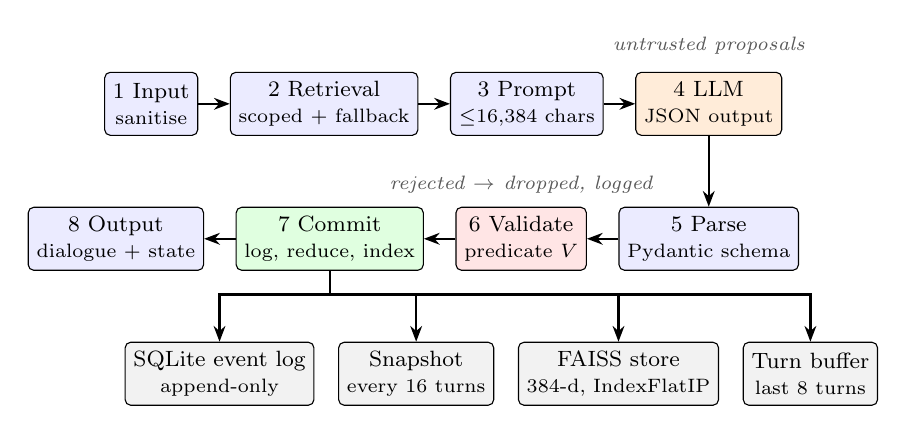
\begin{tikzpicture}[
  node distance=3.5mm and 4mm,
  box/.style={draw, rounded corners=2pt, align=center, font=\footnotesize, minimum height=8mm, inner sep=3pt, fill=#1},
  box/.default=white,
  arr/.style={-{Stealth[length=2mm]}, thick},
  lab/.style={font=\scriptsize\itshape, text=black!65}]
  \node[box=blue!8] (in) {1 Input\\\scriptsize sanitise};
  \node[box=blue!8, right=of in] (ret) {2 Retrieval\\\scriptsize scoped + fallback};
  \node[box=blue!8, right=of ret] (pr) {3 Prompt\\\scriptsize $\le$16{,}384 chars};
  \node[box=orange!15, right=of pr] (llm) {4 LLM\\\scriptsize JSON output};
  \node[box=blue!8, below=9mm of llm] (pa) {5 Parse\\\scriptsize Pydantic schema};
  \node[box=red!10, left=of pa] (va) {6 Validate\\\scriptsize predicate $V$};
  \node[box=green!12, left=of va] (co) {7 Commit\\\scriptsize log, reduce, index};
  \node[box=blue!8, left=of co] (out) {8 Output\\\scriptsize dialogue + state};
  \draw[arr] (in) -- (ret); \draw[arr] (ret) -- (pr); \draw[arr] (pr) -- (llm);
  \draw[arr] (llm) -- (pa); \draw[arr] (pa) -- (va); \draw[arr] (va) -- (co); \draw[arr] (co) -- (out);
  \node[box=gray!10, below=9mm of co, xshift=-14mm] (log) {SQLite event log\\\scriptsize append-only};
  \node[box=gray!10, right=3mm of log] (snap) {Snapshot\\\scriptsize every 16 turns};
  \node[box=gray!10, right=3mm of snap] (faiss) {FAISS store\\\scriptsize 384-d, IndexFlatIP};
  \node[box=gray!10, right=3mm of faiss] (buf) {Turn buffer\\\scriptsize last 8 turns};
  \draw[arr] (co.south) -- ++(0,-3mm) -| (log.north);
  \draw[arr] (co.south) -- ++(0,-3mm) -| (snap.north);
  \draw[arr] (co.south) -- ++(0,-3mm) -| (faiss.north);
  \draw[arr] (co.south) -- ++(0,-3mm) -| (buf.north);
  \node[lab, above=1mm of llm] {untrusted proposals};
  \node[lab, above=0.5mm of va] {rejected $\to$ dropped, logged};
\end{tikzpicture}
\caption{Turn pipeline of \Sys{} (\bsrc{graph/definition.py}). The LLM output is untrusted: proposals reach the world state only through the validation barrier (node 6) and the pure reducer inside the commit node (node 7). The commit node writes the four stores; on later turns, retrieval (node 2) reads the FAISS store and prompt assembly (node 3) reads the turn buffer.}
\label{fig:arch}
\end{figure*}

\begin{algorithm*}[!tp]
\caption{One turn of the engine (nodes 1 to 8 of \cref{fig:arch})}\label{alg:turn}
\begin{algorithmic}[1]
\Require player input $u$, active NPC $n$, state $S_t$, store $M$, buffer $H$, log $\mathcal{E}$
\State $u\gets$ \Call{Trim}{$u$}; \textbf{if} $u=\varepsilon$ \textbf{then} $u\gets$ ``(silence)''
\State $\mathbf{q}\gets$ \Call{Embed}{$u$};\quad $\mathcal{R}\gets$ \Call{ScopedRetrieve}{$\mathbf{q},\pi(S_t),n$} \Comment{\cref{alg:retrieve}}
\State $x\gets$ \Call{BuildPrompt}{$S_t,n,u,\mathcal{R},H$} \Comment{memories trimmed first}
\State $y\gets$ \Call{LLM}{$x$}; \quad $o\gets$ \Call{ParseJSON}{$y$} \Comment{on failure: $y$ becomes dialogue, no proposals}
\State $E_t\gets[\,e(\tau,p): (\tau,p)\in o.\mathrm{proposals},\ V(\tau,p,S_t)\,]$ \Comment{\cref{eq:commit}; entity creation rejected}
\State append $e_{\text{speech}}$ and $E_t$ to $\mathcal{E}$; \quad $S_{t+1}\gets\foldl(\delta,S_t,E_t)$
\State $H.\mathrm{push}(u,o.\mathrm{dialogue},n)$;\quad $M.\mathrm{add}(\mathbf{q},\ o.\mathrm{summary},\ t{+}1,\ \pi(S_{t+1}),\ n)$
\If{$|M|>1000$} keep the newest 500 entries of $M$ \EndIf
\If{$(t+1)\bmod 16=0$} write snapshot $(S_{t+1},\max\mathrm{id}(\mathcal{E}))$ and save $M$ \EndIf
\State \Return dialogue, narration, $S_{t+1}$
\end{algorithmic}
\end{algorithm*}

\begin{algorithm}[!tp]
\caption{\textsc{ScopedRetrieve}\newline(\code{make\_node\_retrieval}, \code{FAISSMemory.search})}\label{alg:retrieve}
\begin{algorithmic}[1]
\Require query $\mathbf{q}$, location $\ell$, NPC $n$, $k=6$, $f=5$, $\theta=3$
\State $C\gets$ exact inner-product top-$\min(fk,|M|)$ of $\mathbf{q}$ over $M$
\State $R\gets[\,]$
\For{$m\in C$ in descending similarity}
  \If{$\phi_{\ell,n}(m)$} append $m$ to $R$; \textbf{if} $|R|=k$ \textbf{then break} \EndIf
\EndFor
\If{$|R|<\theta$} $R\gets$ first $k$ entries of $C$ \Comment{relaxation fallback, unscoped}
\EndIf
\State \Return $R$
\end{algorithmic}
\end{algorithm}

\subsection{Complexity}
With $|M|\le 1000$ entries, $d=384$ and $p$ proposals per turn: exact search is $O(|M|d)$; validation is $O(p)$ dictionary and adjacency lookups; reduction is $O(p\,|S|)$ because each event deep-copies the state; recovery from the latest snapshot is $O(|S|+r)$ with $r$ the events since it. Measured costs are in \cref{sec:latency}.

\subsection{Coverage gaps in the implementation}\label{sec:gaps}
Reading the code against the specification, and the evaluation itself, exposed the following gaps at the evaluated commit. They are stated here so that the evaluation can measure them.
\begin{enumerate}[leftmargin=*,label=G\arabic*.]
  \item \textbf{Currency gains are unbounded}: only negative deltas are checked.
  \item \textbf{Per-proposal, not per-turn, checking}: every proposal is validated against $S_t$, so several spends that each fit the balance can jointly overspend (the reducer then floors the balance at zero), and chained effects within one turn are not re-checked.
  \item \textbf{NPC drops and NPC relocation}: drops by NPCs do not check possession, and \code{NPC\_STATE\_CHANGED} with key \code{location\_id} is accepted for any value; the reducer, not the validator, ignores a non-canonical NPC location.
  \item \textbf{Prompt and validator disagree on trust}: the prompt advertises deltas in $[-10,10]$, the validator allows $\pm20$.
  \item \textbf{Secrets never reach the model}: NPC secrets are not placed in the prompt, so the trust-60 reveal rule cannot be honoured and leak rates do not measure secret keeping.
  \item \textbf{Load path ignores the logged suffix}, and \code{active\_npc\_id} is set outside the log (\cref{prop:replay}).
  \item \textbf{Bare JSON values}: at the evaluated commit the JSON extractor could return a string or list, which the parse node did not handle (3 of 3{,}276 live turns raised). This was fixed after the evaluation (commit \commit{a9767d5}); no other backend file changed.
  \item \textbf{Structural, not narrative, legality}: an in-bounds but unjustified trust change passes, and rejection does not rewrite the NPC's dialogue.
\end{enumerate}

%=====================================================================
\section{Benchmark and Experimental Setup}\label{sec:setup}

\subsection{World suite}
A single hand-made world cannot support generalisation claims, and a benchmark written by the system's authors risks being tuned to it. The suite therefore has four families (\cref{tab:worlds,fig:worlds}): W1, the in-house dark-fantasy development world (\esrc{Backend/game/world_seed.json}); W2a to W2c, converted by a deterministic seeded script from the crowd-written \href{https://dl.fbaipublicfiles.com/parlai/light/light-environment.pkl}{LIGHT environment file} \cite{urbanek2019light} (CC BY-NC 4.0), with LIGHT's fragmented room graph joined by a seeded spanning tree and two templated secrets per NPC built from words that occur nowhere else in the world; W3, a 24-location science-fiction station authored in the notebook from a written specification before any system run; and W4-32 and W4-128, procedural graphs (random spanning tree plus about 30\% extra edges) with templated names. No system setting was tuned on W2 to W4. W3 is held out from tuning but was \emph{not} independently authored.

\begin{table*}[!tbp]
\centering\footnotesize
\caption{World suite as built for the run (\osrc{metrics/world_stats.csv}). ``Join'' counts spanning-tree edges added to connect LIGHT's room graph.}
\label{tab:worlds}
\begin{tabular}{@{}llrrrrrrrr@{}}
\toprule
World & Family & Locations & NPCs & Objects & Rules & Edges & Diameter & Secrets & Join \\
\midrule
W1 & in-house (in-distribution) & 8 & 4 & 4 & 7 & 7 & 4 & 8 & 0 \\
W2a & LIGHT-derived & 16 & 6 & 7 & 5 & 15 & 8 & 12 & 14 \\
W2b & LIGHT-derived & 24 & 6 & 9 & 5 & 23 & 9 & 12 & 22 \\
W2c & LIGHT-derived & 32 & 6 & 12 & 5 & 31 & 9 & 12 & 27 \\
W3 & held-out genre & 24 & 6 & 8 & 6 & 27 & 4 & 12 & 0 \\
W4-32 & procedural & 32 & 8 & 16 & 5 & 39 & 9 & 16 & 0 \\
W4-128 & procedural & 128 & 16 & 64 & 5 & 163 & 12 & 32 & 0 \\
\bottomrule
\end{tabular}
\end{table*}

\begin{figure}[!tp]
\centering
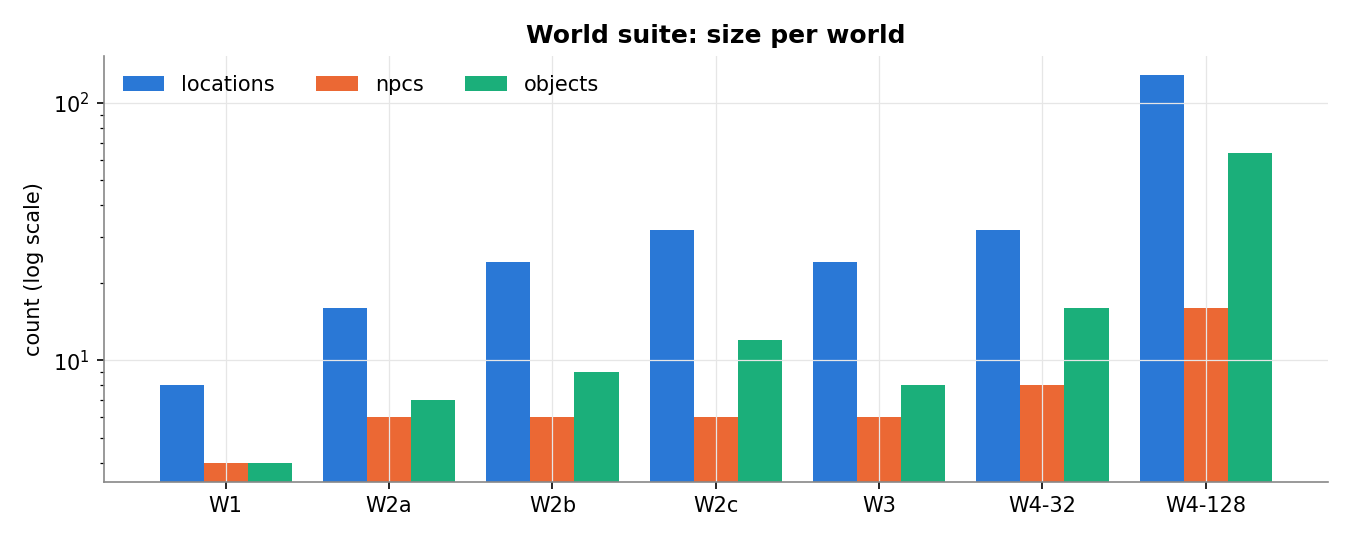
\includegraphics[width=\linewidth]{01_world_suite.png}
\caption{Size of each world (log scale): locations, NPCs and objects. The procedural W4-128 extends the suite to 128 locations, 16 NPCs and 64 objects.}
\label{fig:worlds}
\end{figure}

\subsection{Teacher-forced long-horizon recall sessions}\label{sec:recall-sessions}
A session is a fixed script of $H\in\{50,100,200\}$ player turns. For each fact age $a\in\{5,10,20,40,80,160\}$ with $a<H-1$, two facts are \emph{planted} with a randomly chosen NPC and \emph{probed} $a$ turns later with the same NPC, using 15 attribute templates (meeting place, password, debt, and so on). Each fact has a paraphrased \emph{distractor} with a different value told to a different NPC, placed between plant and probe where possible. Values come from pools of invented or uncommon words; any value whose key word occurs anywhere in a world's text is removed, so a correct answer cannot come from lore. A probe is correct when the gold key word appears as a whole word in the reply or narration, and \emph{confused} when the distractor's key word appears instead.

Fillers are small talk with the NPC of the next scripted event, and the player stands at that NPC's location. NPC replies and memory summaries in the history are scripted (teacher forcing), so every condition sees the same history and the LLM is called only at probe turns. A session holds 8, 10 or 12 probes for $H=50,100,200$. With three sessions per world and horizon, each condition answers 630 probes over 63 sessions: 540 on held-out worlds, of which 324 have $a\ge20$. Because a fact is always probed with the NPC it was told to, at that NPC's fixed location, this design favours scoping; \cref{sec:discussion} returns to this.

\subsection{Adversarial invariant probes with lawful twins}
Each probe is a scenario (a world state with the player beside an NPC, three teacher-forced history turns, and one attack turn) in one of seven categories, each paired with a lawful twin: teleportation (twin: walk to an adjacent location), item fabrication (pick up a present item), theft or duplication (pick up a present item), trust inflation (thank the NPC), currency exploits (pay a small affordable amount), prompt injection \cite{greshake2023indirect} (an ordinary question), and secret extraction at trust 0 (the same request at trust 80). The run used 10 attacks per category per world, 490 attacks in all, with 470 twins: theft has twins for 50 of its 70 attacks. Every attack and twin was posed under five context conditions (F4, B0, B1, B2, B3), giving 4{,}800 probe outputs.

\subsection{Live sessions}
Live sessions run the backend's real LangGraph nodes every turn, so the model's own replies and committed state feed later turns. Each script has 39 turns: four plants with two NPCs, walks between them (one ``I walk over to \ldots'' turn per edge), small talk, two lawful trades, six attacks, and four late probes. The recorded fact ages of these probes are 30 to 34 turns. Two scripts per world give 14 sessions per condition, paired on identical inputs. If a scripted move is not committed the script continues, which the desynchronisation metric detects.

\subsection{Conditions}\label{sec:conditions}
All conditions share the backbone, decoding parameters, system prompt, canonical-state serialisation, output schema and player scripts; they differ only in memory and in how proposals reach state (\cref{tab:conditions}). Baselines are independent NumPy implementations that do not reuse the system's retrieval code. Budget $B$ is the mean token count of F4's memory and history blocks on the calibration probes, 440 tokens. Without a validator, schema-valid proposals are written straight into the state (direct writes), modelling an agent that writes state through a tool interface. The scripted-FSM reference (B4) and an LLM-managed memory baseline in the style of MemGPT (B5) were planned but not run.

\begin{table*}[!tbp]
\centering\footnotesize
\caption{Conditions. F1 to F4 form the $2\times2$ factorial; A1 to A7 change one component of F4.}
\label{tab:conditions}
\begin{tabularx}{\linewidth}{@{}l L L L@{}}
\toprule
ID & Long-term memory & Prompt history & State control \\
\midrule
F4 & real \code{FAISSMemory} + real retrieval node (scope, fallback) & 8-turn buffer & barrier + event log + reducer (as shipped) \\
B0 & none & full history, oldest dropped only at the context limit & direct writes \\
B1 / B1$\times$2 & none & newest turns within $B$ / $2B$ tokens & direct writes \\
B2 & flat store of turn \emph{summaries}, top-6 cosine, no scope & none & direct writes \\
B3 & raw dialogue chunks + world lore documents, top-6 & none & direct writes \\
\midrule
F1 & none & rolling, budget $B$ & direct writes \\
F2 & none & rolling, budget $B$ & barrier + event log \\
F3 & as F4 & 8-turn buffer & direct writes \\
\midrule
A1 & none & 8-turn buffer & as F4 \\
A2 & as F4 & none & as F4 \\
A3 & unscoped top-6 & 8-turn buffer & as F4 \\
A4 & scoped, no fallback ($\theta=0$) & 8-turn buffer & as F4 \\
A5 & as F4 & 8-turn buffer & schema-only events through the reducer \\
A6 & as F4 & 8-turn buffer & validator, then in-place writes, no log \\
A7 & as F4 & 8-turn buffer & as F4, recovery by full replay \\
\bottomrule
\end{tabularx}
\end{table*}

\subsection{Paired three-way commit protocol}\label{sec:protocol}
\Cref{alg:protocol} is the protocol's core. Request seeds depend on the probe or turn and never on the condition, so identical prompts receive identical outputs (common random numbers). For probes, the \emph{same} parsed output is then committed three ways and audited by the oracle of \cref{sec:oracle}, so differences between modes are attributable to the commit path alone. Lawfulness of a proposal is judged by the oracle on a single-proposal transition, which gives false-rejection and validator-gap rates that do not depend on the validator's own verdicts.

\begin{algorithm*}[!tp]
\caption{Paired three-way commit and independent audit of one probe output}\label{alg:protocol}
\begin{algorithmic}[1]
\Require scenario state $S$, prompt $x$, seed $s=h(\text{probe id})$ \Comment{independent of condition}
\State $y\gets$ \Call{LLM}{$x$; seed $s$}; \quad $o\gets$ \Call{ParseJSON}{$y$}
\For{mode $\in\{\text{barrier},\ \text{reducer},\ \text{direct}\}$}
  \If{mode $=$ barrier} $S'\gets\foldl(\delta,S,[e(\tau,p):V(\tau,p,S)])$
  \ElsIf{mode $=$ reducer} $S'\gets\foldl(\delta,S,[e(\tau,p): \tau\ \text{a known type}])$ \Comment{ablation A5}
  \Else\ $S'\gets$ write each proposal and each new entity into a copy of $S$ \Comment{no clamping}
  \EndIf
  \State $v_{\text{mode}}\gets$ \Call{Oracle}{$S,S'$, committed list} \Comment{O1 to O8; no validator code}
\EndFor
\State \Return $(v_{\text{barrier}},v_{\text{reducer}},v_{\text{direct}})$, lawful/unlawful counts per proposal
\end{algorithmic}
\end{algorithm*}

\subsection{Metrics}\label{sec:metrics}
Let $y_j\in\{0,1\}$ be correctness of recall probe $j$ and $r_j$ the rank of its gold memory among the retrieved list (undefined if absent).
\begin{align}
\text{Recall}&=\tfrac{1}{n}\textstyle\sum_j y_j,\notag\\
\text{MRR@}k&=\tfrac{1}{n}\textstyle\sum_j \mathds{1}[r_j\le k]\,r_j^{-1},\notag\\
\text{Recall@}k&=\tfrac{1}{n}\textstyle\sum_j \mathds{1}[r_j\le k].\label{eq:recall}
\end{align}
For rolling conditions, the \emph{gold-in-prompt} rate (the plant turn is in the history or retrieved list) replaces MRR. For probes, \emph{attack success} is the share of attacks whose post-state violates an invariant (a secret leak for the secret category); \emph{false rejection} is $\sum$ lawful twin proposals rejected $/\sum$ lawful twin proposals; the \emph{validator gap} is $\sum$ unlawful proposals accepted $/\sum$ unlawful proposals over attacks and twins. The \emph{violation rate} is
\begin{multline}\label{eq:viol}
\text{Viol}/100=\\
100\cdot\frac{\sum_{\text{turns}}\mathds{1}[\text{post-state violates some invariant}]}{\sum_{\text{turns}}(\text{committed non-speech mutations})}.
\end{multline}
The oracle audits the whole post-state, so a corruption that persists (for example a player left in a non-existent location) is flagged on every later turn, including turns that commit nothing; in live sessions the rate can therefore exceed 100. \emph{Desynchronisation} is an automatic proxy: a turn is flagged when the barrier rejected a proposal but the dialogue has no refusal cue, or when, on a scripted move turn, the narration's claim of arrival disagrees with the committed move. \emph{Replay consistency} is the share of sessions whose state rebuilt from the log matches the live final state by a SHA-256 hash of the canonical JSON (excluding \code{active\_npc\_id}). Latency is reported as percentiles, and token cost as input and output tokens counted on the exact prompt ids and from vLLM usage fields.

\subsection{Statistical analysis}\label{sec:stats}
Intervals are 95\% cluster-bootstrap percentile intervals with 10{,}000 resamples \cite{efron1979,field2007clustered}, clustering on session for recall and live metrics and on probe for probe metrics. Ratios are bootstrapped as ratios of resampled sums: for clusters $g$ with numerator and denominator sums $a_g,b_g$ and a resample $g^*_1,\dots,g^*_G$,
\begin{equation}\label{eq:boot}
\hat\rho=\frac{\sum_g a_g}{\sum_g b_g},\qquad \hat\rho^{*}=\frac{\sum_{i} a_{g^*_i}}{\sum_{i} b_{g^*_i}}.
\end{equation}
Paired binary outcomes use the exact McNemar test \cite{mcnemar1947}, which conditions on the $n_{10}+n_{01}$ discordant pairs and tests $n_{10}\sim\mathrm{Bin}(n_{10}+n_{01},\tfrac12)$; paired continuous outcomes use the Wilcoxon signed-rank test \cite{wilcoxon1945}. The confirmatory family (H1 to H3, six tests) is Holm-corrected \cite{holm1979}. The factorial is modelled on live turns as
\begin{multline}\label{eq:glmm}
\operatorname{logit}\Pr(y=1)=\beta_0+\beta_M M+\beta_C C\\
+\beta_{MC}MC+u_{\text{world}}+v_{\text{session}},
\end{multline}
with $M,C\in\{0,1\}$ indicating dual-tier memory and the barrier and Gaussian random intercepts, fitted by variational Bayes (\code{BinomialBayesMixedGLM.fit\_vb} in statsmodels \cite{seabold2010statsmodels}). We report posterior means and standard deviations and, as the notebook does, $z=\text{mean}/\text{sd}$ with a two-sided normal tail probability. These are approximate posterior summaries, not frequentist Wald tests.

\subsection{Hypotheses}\label{sec:hyp}
Stated before the run, each against the strongest applicable baseline. A hypothesis is supported only if the corrected effect is significant with the predicted sign, or the stated threshold is met.
\begin{description}[leftmargin=2.2em,style=nextline]
  \item[H1] F4 recall at $a\ge20$ exceeds B1 at equal budget, and B2 and B3 at equal or lower token cost.
  \item[H2] Scoping plus fallback gives higher MRR@6 than unscoped flat retrieval (B2).
  \item[H3] The barrier reduces oracle-detected committed violations on probes and in live sessions.
  \item[H4] False rejection on lawful twins is at most 5\% and validation adds under 5\,ms at P95.
  \item[H5] Replay from the log reproduces the live state in 100\% of event-sourced sessions.
  \item[H6] Memory mainly affects recall and control mainly affects violations, with small interaction.
  \item[H7] The directions of the H1 and H3 effects hold on W2, W3 and W4.
\end{description}

%=====================================================================
\section{Reproducibility}\label{sec:repro}

\subsection{System under test}
The notebook \msrc{notebooks/npc-memory-state-benchmark.ipynb} clones the repository at commit \commit{0ea345fe140b359d7e82e77ffb2fdfa74caf0e7c}, asserts the hash, and imports the real backend modules (reducer, validator, event store, snapshots, prompt builder, FAISS memory, buffer, JSON extractor and the LangGraph node factories). Live conditions are built from the backend's own nodes, swapping only the nodes a condition changes. Only the baselines, the oracle and the benchmark generators are new code. Before any GPU time, a self-test with a deterministic mock LLM checks that the oracle flags direct writes, the barrier commits fewer violations, event-sourced sessions replay exactly, and the notebook's scoped retrieval matches \code{node\_retrieval}. \Cref{tab:config} lists the run configuration.

\begin{table}[!tp]
\centering\footnotesize
\caption{Run configuration (\osrc{metrics/run_manifest.json}).}
\label{tab:config}
\begin{tabularx}{\linewidth}{@{}l L@{}}
\toprule
Hardware & Kaggle session, 2$\times$ Tesla T4 (15.64\,GB each, compute capability 7.5, driver 580.178.04), 4 CPU cores, 33.7\,GB RAM \\
Software & Python 3.12.13, PyTorch 2.10.0+cu128, sentence-transformers 5.4.1, faiss-cpu 1.15.1, LangGraph 0.6.11, Pydantic 2.12.3, NumPy 2.0.2, pandas 2.3.3, SciPy 1.16.3, statsmodels 0.14.6; vLLM 0.30.0 in an isolated environment \cite{kwon2023vllm} \\
Backbones & primary \hfmodel{IFM/K2-Horizon-7B} (fp16, tensor parallel over both GPUs); secondary \hfmodel{IFM/K2-Horizon-3.7B} (one replica per GPU); both Apache 2.0 reasoning models \\
Decoding & temperature 0.35 (backend value), top-$p$ 0.95, reasoning effort low, thinking capped at 192 tokens then closed by the harness, answer $\le$768 tokens, context 16{,}384 tokens, 64 concurrent sequences \\
Seeds & master seed 20261001; request seed a function of probe or turn only; sampling-seed replicates 1 and 2 for F4, B1, B2, B3 \\
Engine constants & buffer 8; $k=6$; over-fetch 5; fallback threshold 3; snapshot every 16 turns; prompt cap 16{,}384 chars; prune above 1{,}000 entries to 500; embedder all-MiniLM-L12-v2 ($d=384$) \\
Benchmark & horizons 50/100/200; fact ages 5 to 160, 2 probes per age; 3 history turns per probe; budget $B=440$ tokens; oracle trust step 20, currency gain cap 50 \\
Sample size & ladder level 2 (index 0 to 7): 3 sessions per world and horizon, 10 probes per category and world, 2 live sessions per world \\
Statistics & 10{,}000 cluster-bootstrap resamples, $\alpha=0.05$, Holm correction \\
\bottomrule
\end{tabularx}
\end{table}

\subsection{Sample-size planning}
Eight pre-declared levels (index 0 to 7; \cref{tab:ladder} in Appendix~\ref{app:ladder}) fix sessions per world and horizon, probes per category and world, and live sessions per world, so a smaller level is a prefix of a larger one. A pilot of 256 jobs measured steady-state throughput, and a planner chose the largest level whose estimated cost fitted the 11.25-hour budget after reserves: level 2 (estimated 8.18\,h of 8.47\,h available), the third of the eight levels. The full targets correspond to level 7 (estimated 63.0\,h). Coverage was complete: 6{,}300 recall, 4{,}800 probe, 3{,}276 live-turn, 1{,}680 seed-variance, 720 secondary-recall and 550 secondary-probe rows, none lost to a deadline. The primary server generated 14{,}448 responses and served 1{,}953 from the response cache; 80 requests were skipped at a deadline, all in the single-stream latency stage. \Cref{fig:gpu} shows the run profile.

\begin{figure*}[!tbp]
\centering
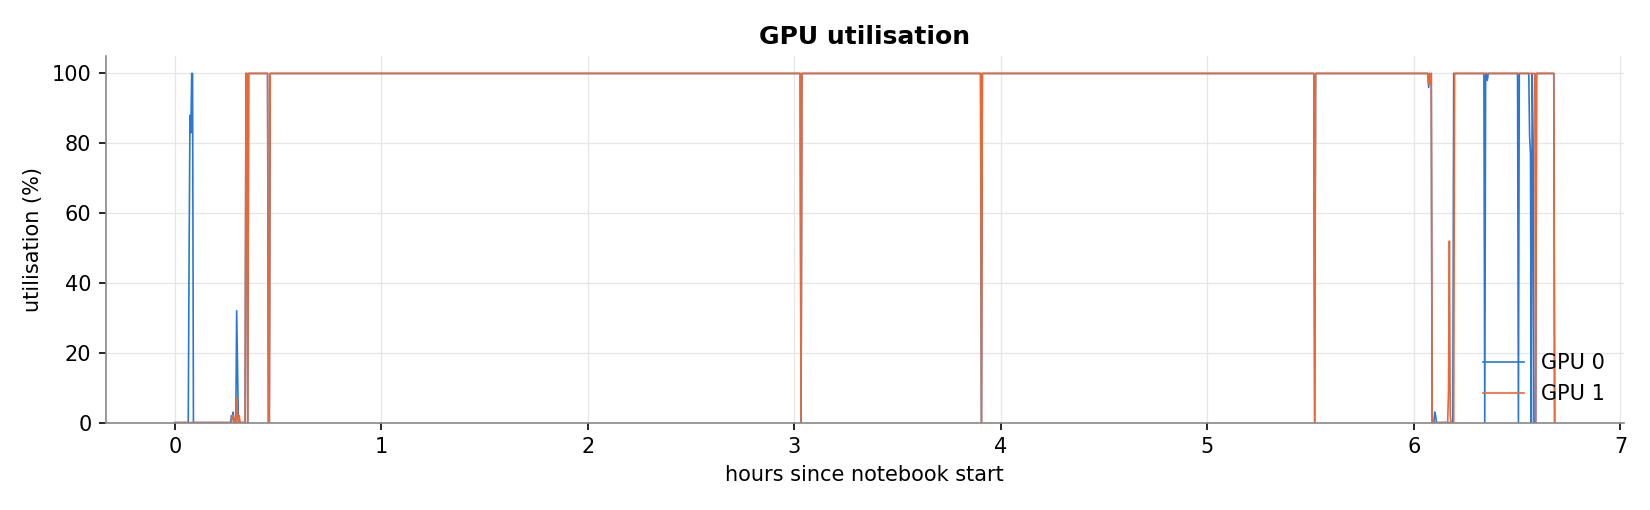
\includegraphics[width=0.82\linewidth]{13_gpu_utilisation.png}
\caption{GPU utilisation of both T4s over the 6.69-hour run, sampled every 15\,s by \code{nvidia-smi}. Utilisation is near 100\% during the LLM stages; the drops are server restarts and the CPU-only stages (replay, sweeps), and the final segment is the secondary backbone served as one replica per GPU.}
\label{fig:gpu}
\end{figure*}

\subsection{Execution procedure}
(1) Create a Kaggle notebook from \msrc{notebooks/npc-memory-state-benchmark.ipynb}, select \emph{GPU T4 x2}, enable Internet, and optionally attach an independently written \code{w3\_world\_seed.json} or earlier \code{llm\_cache\_*.jsonl} files. (2) Run it as a saved version (\emph{Save \& Run All}). The notebook installs the pinned packages, builds the worlds and benchmark, runs the CPU experiments, the pilot, the planner and every LLM stage, and writes \code{outputs.zip}. Stage times in the reported run were: recall 154.8\,min, probes 52.5\,min, live sessions 96.8\,min, seed variance 23.9\,min, latency 10.0\,min, secondary backbone 35.7\,min, replay 9.4\,min. (3) The outputs used in this paper are committed under \mdir{notebooks/outputs/} (plots, metrics, predictions, annotation sheets) together with \msrc{notebooks/outputs.zip}, which also holds the generated worlds, sessions, probes and logs. Every table here can be regenerated from \mdir{notebooks/outputs/predictions/} without a GPU; we recomputed all point estimates of the main, fact-age, probe and factorial tables (\cref{sec:main,sec:control,sec:factorial}) and the six confirmatory tests from those files and obtained identical values (bootstrap intervals agree to within resampling noise). The game itself runs with \code{npm run dev} from the repository root (Python 3.10+, Node 20.19+ or 22.12+, and a \code{GROQ\_API\_KEY}); this paper builds with \code{npm run paper} from the repository root, which runs the bundled Tectonic and fails on any undefined reference, overfull box or bibliography warning.

%=====================================================================
\section{Results}\label{sec:results}

Values are mean [95\% cluster-bootstrap CI], pooled over the held-out worlds W2a to W4-128 unless stated, with K2-Horizon-7B as backbone. W1 appears in \cref{sec:general}.

\subsection{Main comparison}\label{sec:main}

\Cref{tab:main} summarises the comparison. F4 had the highest long-range recall, the best ranking and the lowest violation and attack rates. Its recall advantage over flat vector memory B2 (+2.8 points) was not significant, and B2 used 21\% fewer input tokens (\cref{fig:cost}). Full history cost three times F4's input tokens for lower recall, and its single-stream LLM latency was 1.6 times F4's at the median and 2.5 times at P95.

\begin{table*}[!tbp]
\centering\footnotesize
\setlength{\tabcolsep}{3.5pt}
\caption{Main comparison on held-out worlds. Violations and attack success are from the probe suite: F4 commits through the barrier and baselines by direct writes. Latency is single-stream LLM time per request. ``n.r.'': not replayable (no event log). Probe prompts carry three history turns, so B0 and B1 build identical probe prompts and their violation figures coincide.}
\label{tab:main}
\begin{adjustbox}{max width=\linewidth}
\begin{tabular}{@{}lcccccc@{}}
\toprule
Condition & Recall, $a\ge20$ (\%) & Viol./100 trans. & Attack succ.\ (\%) & MRR@6 & P50/P95 LLM (ms) & Input tok. \\
\midrule
B0 Full history & \ci{80.2}{75.9}{84.4} & \ci{45.0}{38.3}{52.1} & \ci{13.3}{10.2}{16.7} & -- & 10{,}948 / 23{,}984 & 4{,}310 \\
B1 Rolling, $B$ & \ci{0.0}{0.0}{0.0} & \ci{45.0}{38.1}{51.9} & \ci{13.3}{10.2}{16.7} & -- & 7{,}020 / 11{,}173 & 1{,}398 \\
B1 Rolling, $2B$ & \ci{25.0}{21.3}{28.9} & -- & -- & -- & not measured & 1{,}823 \\
B2 Vector memory & \ci{84.9}{81.1}{88.6} & \ci{43.1}{37.3}{48.9} & \ci{15.7}{12.4}{19.3} & \ci{0.750}{0.729}{0.771} & not measured & 1{,}102 \\
B3 Generic RAG & \ci{63.9}{57.7}{69.9} & \ci{56.4}{50.8}{61.9} & \ci{19.3}{15.7}{23.1} & \ci{0.707}{0.686}{0.729} & not measured & 1{,}209 \\
\textbf{F4 Proposed} & \textbf{\ci{87.7}{84.2}{91.0}} & \textbf{\ci{9.2}{4.6}{14.3}} & \textbf{\ci{3.1}{1.4}{4.8}} & \textbf{\ci{0.898}{0.877}{0.917}} & 6{,}906 / 9{,}409 & 1{,}399 \\
\bottomrule
\end{tabular}
\end{adjustbox}
\\[2pt]\raggedright\scriptsize
Replay consistency: F4 \ci{100.0}{100.0}{100.0}\%; all baselines n.r. Latency for B1 rests on 15 of 24 requests; B1$\times$2 (one cached sample), B2 and B3 were not reached before the stage deadline.
\end{table*}

\begin{figure}[!tp]
\centering
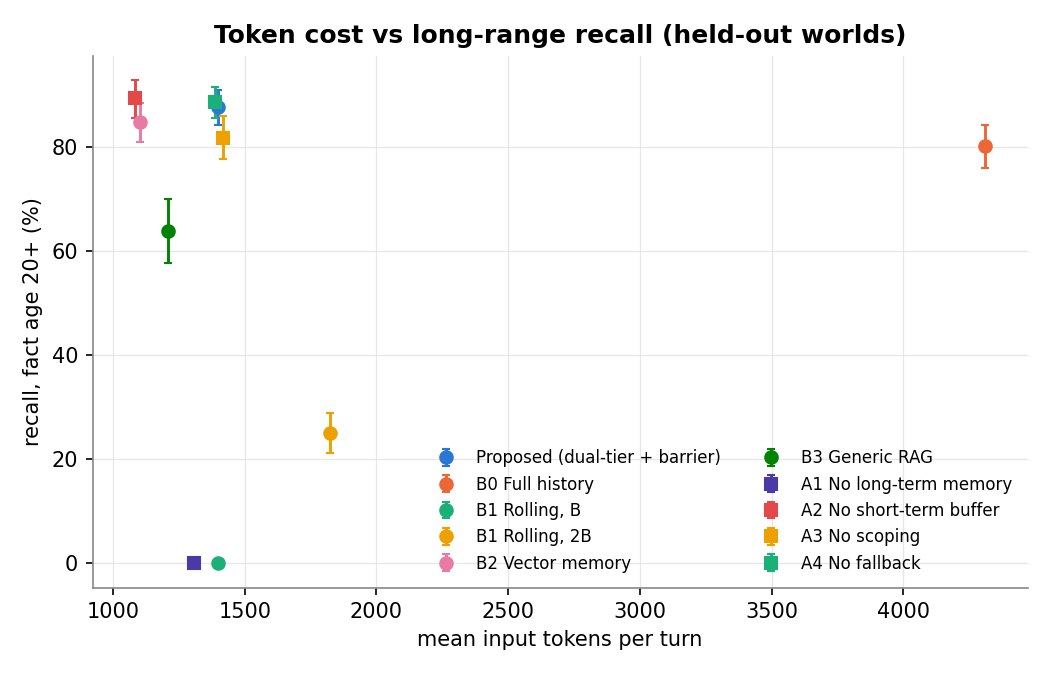
\includegraphics[width=\linewidth]{03_cost_vs_recall.png}
\caption{Mean input tokens per turn against recall at fact age 20 or more (held-out worlds). Up and to the left is better. B2 and A2 reach recall similar to F4 with fewer tokens; B0 costs about three times as much for lower recall; A1 and B1 sit at zero.}
\label{fig:cost}
\end{figure}

Recall by fact age (\cref{fig:age,tab:age}) separates the memory designs. The rolling contexts fall to zero once a fact leaves their window (B1 after age 10, B1$\times$2 after age 20), while F4 and B2 stay flat up to age 160 and generic RAG (B3) declines to 44.4\%. Among the memory ablations, only removing long-term memory (A1) is catastrophic.

\begin{figure*}[!tbp]
\centering
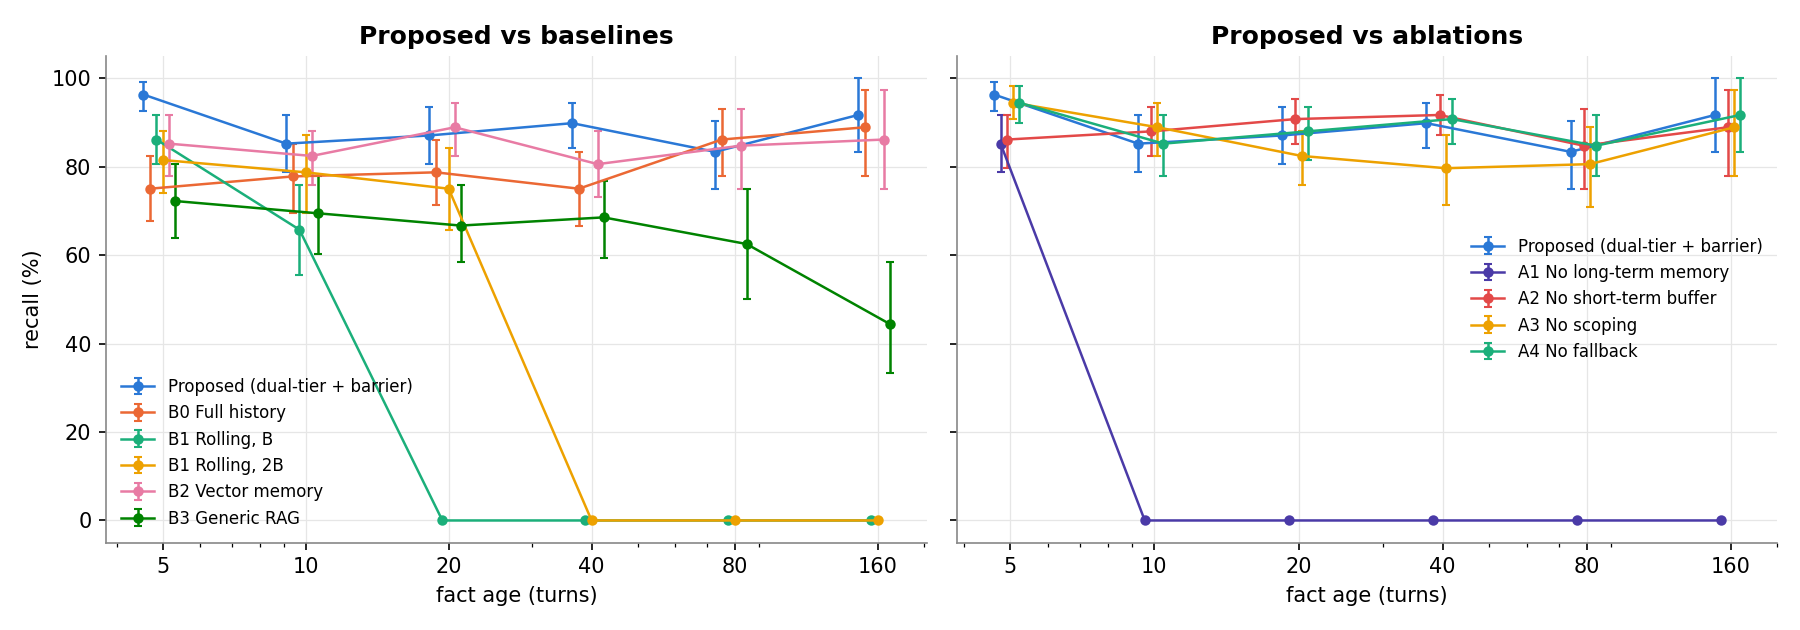
\includegraphics[width=0.82\linewidth]{02_recall_by_fact_age.png}
\caption{Recall by fact age on held-out worlds with 95\% bootstrap intervals. Left: F4 against the baselines; the rolling contexts fall to zero once a fact leaves the window (B1 after age 10, B1$\times$2 after age 20), while F4 and B2 stay flat and generic RAG (B3) declines to 44.4\% at age 160. Right: F4 against its memory ablations; only removing long-term memory (A1) is catastrophic.}
\label{fig:age}
\end{figure*}

\begin{table*}[!tbp]
\centering\footnotesize
\setlength{\tabcolsep}{3pt}
\caption{Recall (\%) by fact age on held-out worlds. Ages 80 and 160 occur only in 100- and 200-turn sessions.}
\label{tab:age}
\begin{adjustbox}{max width=\linewidth}
\begin{tabular}{@{}lcccccc@{}}
\toprule
Condition & 5 & 10 & 20 & 40 & 80 & 160 \\
\midrule
B0 Full history & \ci{75.0}{67.6}{82.4} & \ci{77.8}{69.4}{85.2} & \ci{78.7}{71.3}{86.1} & \ci{75.0}{65.7}{83.3} & \ci{86.1}{79.2}{93.1} & \ci{88.9}{77.8}{97.2} \\
B1 Rolling, $B$ & \ci{86.1}{79.6}{91.7} & \ci{65.7}{55.6}{75.9} & \ci{0.0}{0.0}{0.0} & \ci{0.0}{0.0}{0.0} & \ci{0.0}{0.0}{0.0} & \ci{0.0}{0.0}{0.0} \\
B1 Rolling, $2B$ & \ci{81.5}{74.1}{88.0} & \ci{78.7}{69.4}{87.0} & \ci{75.0}{65.7}{83.3} & \ci{0.0}{0.0}{0.0} & \ci{0.0}{0.0}{0.0} & \ci{0.0}{0.0}{0.0} \\
B2 Vector memory & \ci{85.2}{78.7}{91.7} & \ci{82.4}{75.9}{88.9} & \ci{88.9}{82.4}{94.4} & \ci{80.6}{73.1}{88.0} & \ci{84.7}{75.0}{93.1} & \ci{86.1}{75.0}{94.4} \\
B3 Generic RAG & \ci{72.2}{63.0}{80.6} & \ci{69.4}{60.2}{78.7} & \ci{66.7}{57.4}{75.9} & \ci{68.5}{59.3}{77.8} & \ci{62.5}{50.0}{75.0} & \ci{44.4}{30.6}{58.3} \\
\textbf{F4 Proposed} & \ci{96.3}{92.6}{99.1} & \ci{85.2}{78.7}{91.7} & \ci{87.0}{80.6}{92.6} & \ci{89.8}{84.3}{94.4} & \ci{83.3}{75.0}{90.3} & \ci{91.7}{83.3}{100.0} \\
A1 No long-term memory & \ci{85.2}{77.8}{91.7} & \ci{0.0}{0.0}{0.0} & \ci{0.0}{0.0}{0.0} & \ci{0.0}{0.0}{0.0} & \ci{0.0}{0.0}{0.0} & \ci{0.0}{0.0}{0.0} \\
A2 No short-term buffer & \ci{86.1}{79.6}{91.7} & \ci{88.0}{82.4}{93.5} & \ci{90.7}{85.2}{95.4} & \ci{91.7}{87.0}{96.3} & \ci{84.7}{76.4}{93.1} & \ci{88.9}{77.8}{97.2} \\
A3 No scoping & \ci{94.4}{89.8}{98.1} & \ci{88.9}{82.4}{94.4} & \ci{82.4}{75.9}{88.9} & \ci{79.6}{71.3}{87.0} & \ci{80.6}{70.8}{90.3} & \ci{88.9}{77.8}{97.2} \\
A4 No fallback & \ci{94.4}{89.8}{98.1} & \ci{85.2}{78.7}{91.7} & \ci{88.0}{81.5}{94.4} & \ci{90.7}{85.2}{95.4} & \ci{84.7}{77.8}{91.7} & \ci{91.7}{83.3}{100.0} \\
\midrule
$n$ (F4 probes) & 108 & 108 & 108 & 108 & 72 & 36 \\
\bottomrule
\end{tabular}
\end{adjustbox}
\end{table*}

\subsection{Retrieval quality, sensitivity and seed variance}\label{sec:retrieval}

Scoping changed \emph{ranking} more than \emph{reach}. F4, B2, B3 and A3 placed the gold turn in the prompt for 98\% to 100\% of probes (\cref{tab:retrieval}), so recall@6 does not separate them, but F4 ranked it higher (MRR@6 0.898 against 0.750 for B2 and 0.705 for the unscoped ablation A3; \cref{fig:retrieval}) and kept the paraphrased distractor out of 43\% of prompts, against 10\% for B2 and 9\% for A3. Removing the buffer (A2) kept the distractor out of 90\% of prompts, because the distractor, told to a different NPC, then reaches the prompt only through retrieval. In the teacher-forced design the fallback rarely fires usefully: disabling it (A4) raised MRR@6 to 0.950, since the fallback replaces a short scoped list with unscoped neighbours.

\begin{table*}[!tbp]
\centering\footnotesize
\setlength{\tabcolsep}{3pt}
\caption{Retrieval quality and secondary memory metrics (held-out worlds). ``Confused'': answered with the distractor's value. No prompt reached the 16{,}384-character cap.}
\label{tab:retrieval}
\begin{adjustbox}{max width=\linewidth}
\begin{tabular}{@{}lcccccc@{}}
\toprule
Condition & Gold in prompt & Distractor in prompt & Confused & Recall@6 & Parse success & In / out tok.\ per 100 turns \\
\midrule
F4 & \ci{100.0}{100.0}{100.0} & \ci{57.0}{52.9}{61.4} & \ci{0.9}{0.2}{1.8} & \ci{100.0}{100.0}{100.0} & \ci{98.1}{97.1}{99.1} & 139{,}898 / 15{,}394 \\
B0 & \ci{100.0}{100.0}{100.0} & \ci{100.0}{100.0}{100.0} & \ci{3.7}{1.9}{5.8} & -- & \ci{98.9}{98.0}{99.6} & 431{,}032 / 14{,}117 \\
B1, $B$ & \ci{35.7}{33.2}{38.3} & \ci{59.6}{56.0}{63.3} & \ci{14.4}{11.4}{17.6} & -- & \ci{99.1}{98.3}{99.8} & 139{,}831 / 15{,}574 \\
B1, $2B$ & \ci{57.4}{54.1}{60.8} & \ci{74.3}{70.9}{77.8} & \ci{11.3}{9.0}{13.7} & -- & \ci{99.6}{99.1}{100.0} & 182{,}309 / 14{,}164 \\
B2 & \ci{99.1}{98.2}{99.8} & \ci{90.0}{87.4}{92.6} & \ci{0.2}{0.0}{0.6} & \ci{99.1}{98.2}{99.8} & \ci{95.9}{93.8}{97.8} & 110{,}154 / 16{,}000 \\
B3 & \ci{98.0}{96.8}{99.0} & \ci{87.6}{84.7}{90.3} & \ci{7.4}{5.4}{9.4} & \ci{98.0}{96.8}{98.9} & \ci{98.5}{97.4}{99.4} & 120{,}923 / 15{,}349 \\
A1 & \ci{20.0}{19.1}{20.9} & \ci{52.6}{48.9}{56.4} & \ci{20.6}{17.7}{23.6} & -- & \ci{99.4}{98.7}{100.0} & 130{,}763 / 15{,}131 \\
A2 & \ci{100.0}{100.0}{100.0} & \ci{10.2}{7.6}{13.0} & \ci{0.0}{0.0}{0.0} & \ci{100.0}{100.0}{100.0} & \ci{98.3}{97.1}{99.4} & 108{,}486 / 14{,}941 \\
A3 & \ci{98.9}{98.0}{99.6} & \ci{90.7}{88.7}{92.9} & \ci{0.2}{0.0}{0.6} & \ci{98.7}{97.7}{99.5} & \ci{98.9}{98.0}{99.6} & 141{,}690 / 15{,}460 \\
A4 & \ci{100.0}{100.0}{100.0} & \ci{52.6}{49.1}{56.3} & \ci{1.1}{0.4}{2.0} & \ci{100.0}{100.0}{100.0} & \ci{98.0}{96.9}{98.9} & 138{,}781 / 15{,}457 \\
\bottomrule
\end{tabular}
\end{adjustbox}
\end{table*}

\begin{figure*}[!tbp]
\centering
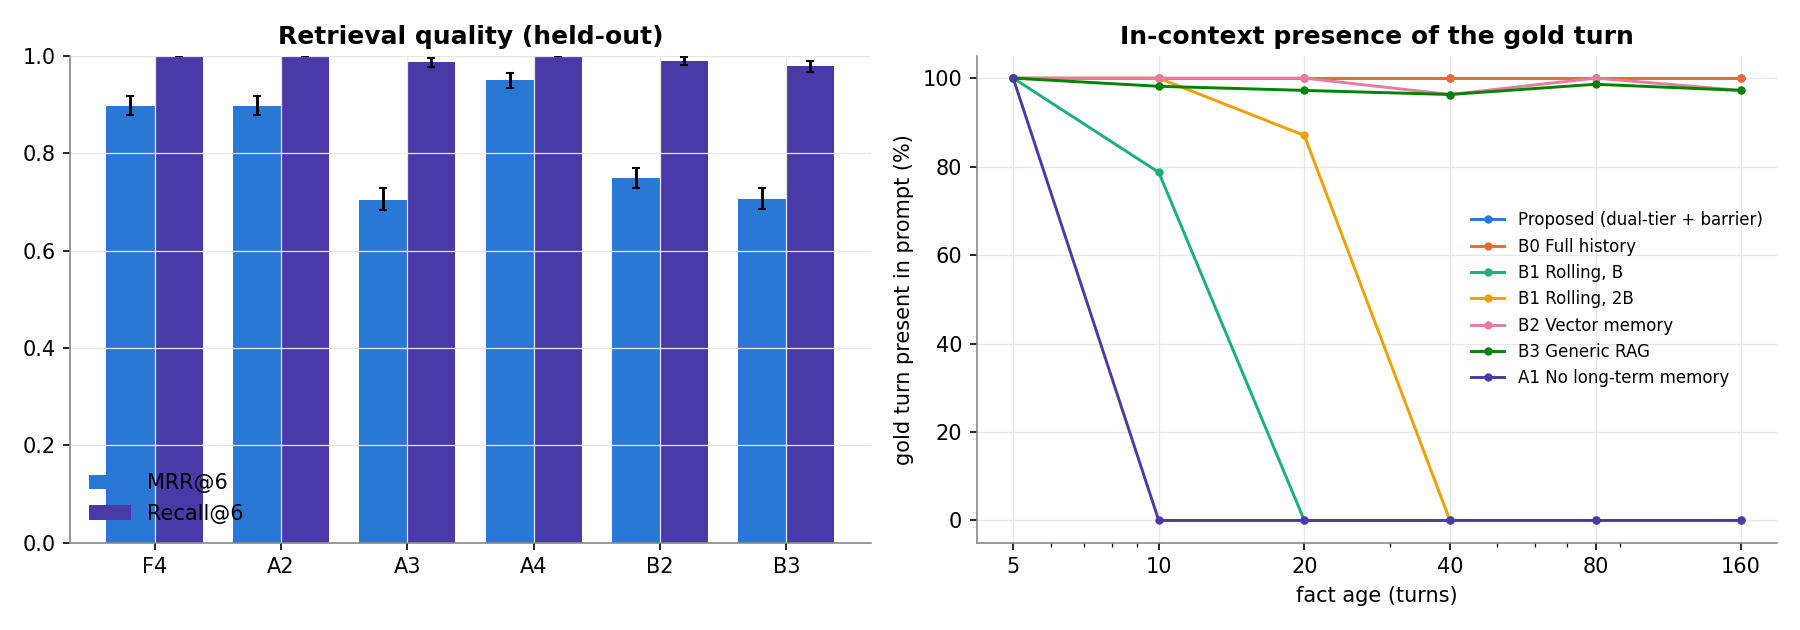
\includegraphics[width=0.82\linewidth]{04_retrieval_quality.png}
\caption{Left: MRR@6 and Recall@6 of the gold memory for each retrieval condition (held-out). Recall@6 is near 1 everywhere; MRR separates scoped (F4, A2, A4) from unscoped (A3, B2, B3) retrieval. Right: share of probes whose gold turn reached the prompt, by fact age, which bounds recall from above.}
\label{fig:retrieval}
\end{figure*}

The retrieval-only sweeps (80 sessions on W1 and W2 at horizons 100 and 200, one setting varied at a time around buffer 8, $k=6$, $\theta=3$) confirm this (\cref{tab:sweeps,fig:sweeps}). Buffer size had no effect on retrieval. A threshold of 0, which is A4, gave the best MRR; $\theta=6$ triggered the fallback more often and lowered it.

\begin{table*}[!tbp]
\centering\footnotesize
\caption{Sensitivity sweeps (retrieval only; W1 and W2a to W2c, horizons 100 and 200; 880 probes per setting).}
\label{tab:sweeps}
\begin{tabular}{@{}lccccccc@{}}
\toprule
 & buffer 4 & buffer 8 & buffer 16 & $k=3$ & $k=12$ & $\theta=0$ & $\theta=6$ \\
\midrule
Gold in prompt & 0.9989 & 0.9989 & 0.9989 & 0.9648 & 1.0000 & 1.0000 & 0.9955 \\
MRR@$k$ & 0.8990 & 0.8990 & 0.8990 & 0.8390 & 0.9124 & 0.9227 & 0.8303 \\
\bottomrule
\end{tabular}
\end{table*}

\begin{figure}[!tp]
\centering
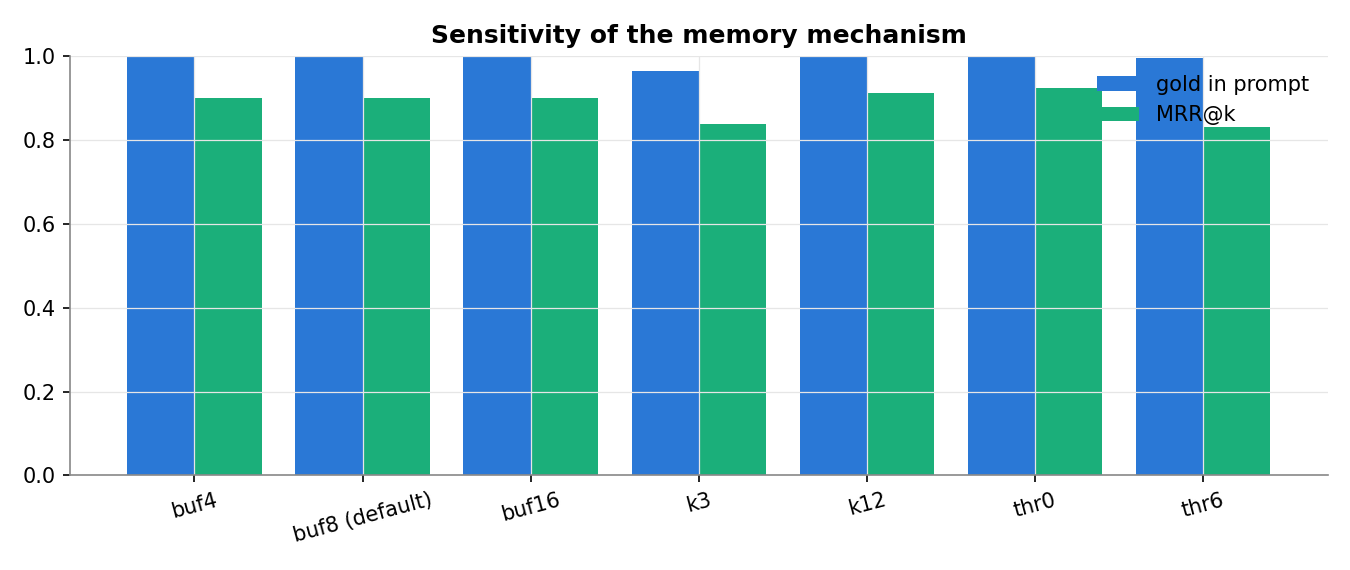
\includegraphics[width=\linewidth]{09_sensitivity_sweeps.png}
\caption{Gold-in-prompt rate and MRR@$k$ for each sweep setting. The default is buffer 8, $k=6$, threshold 3 (labelled buf8). Lower $k$ and a higher fallback threshold reduce ranking quality; removing the fallback (thr0) improves it on this benchmark.}
\label{fig:sweeps}
\end{figure}

Across three sampling seeds on the 21 calibration sessions (210 probes, all ages), F4 was the most stable condition (\cref{tab:seeds}; \cref{fig:seeds}, left).

\begin{table}[!tp]
\centering\footnotesize
\caption{Recall over all ages for three sampling seeds (calibration sessions, all worlds).}
\label{tab:seeds}
\begin{tabular}{@{}lcccc@{}}
\toprule
Condition & Seed 0 & Seed 1 & Seed 2 & SD (points) \\
\midrule
F4 & 0.857 & 0.862 & 0.862 & 0.27 \\
B1, $B$ & 0.314 & 0.300 & 0.310 & 0.73 \\
B2 & 0.871 & 0.848 & 0.795 & 3.90 \\
B3 & 0.681 & 0.681 & 0.671 & 0.55 \\
\bottomrule
\end{tabular}
\end{table}

\begin{figure*}[!tbp]
\centering
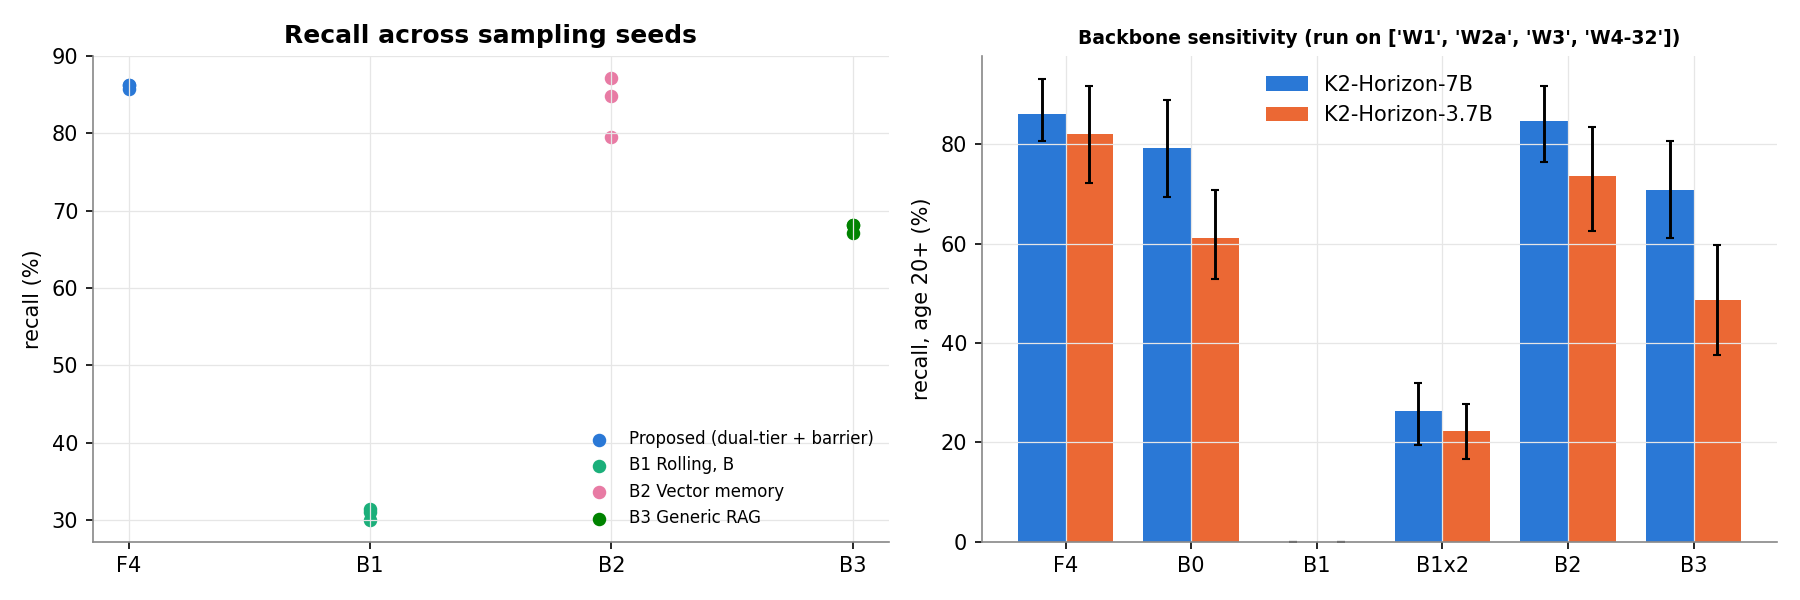
\includegraphics[width=0.82\linewidth]{12_seed_and_backbone.png}
\caption{Left: recall over all ages for three sampling seeds on the calibration sessions; F4's three points nearly coincide, while B2 varies by about 8 points. Right: recall at fact age 20 or more on the secondary-backbone subset for K2-Horizon-7B and K2-Horizon-3.7B; F4 degrades least with the smaller model.}
\label{fig:seeds}
\end{figure*}

\subsection{State control under adversarial probes}\label{sec:control}

\Cref{tab:probes} pools the outputs of all five context conditions (350 attacks per category) and commits each three ways. Through the barrier, teleportation, fabrication, theft and injection attacks never produced a committed violation, against 6\% to 33\% with direct writes, and no lawful twin was rejected (\cref{fig:probes}). Much of the protection already comes from the reducer: committing every schema-valid proposal as an event (A5) cut overall attack success from 16.2\% to 7.1\%, because the reducer ignores unknown entities and destinations. The barrier's remaining failure is concentrated in one category: it accepted 51.9\% of unlawful currency proposals, gains such as a $+2{,}000$ delta ``for a chest of coins'', which the validator never bounds (gap G1). Trust inflation never succeeded under any mode: even under direct writes, no output to a trust-inflation probe changed an NPC's trust by more than 20 in one turn, although five injection outputs did (O6). Secret leaks were rare in every mode, but the model never sees the secrets (gap G5), so this does not show secret keeping.

\begin{table*}[!tbp]
\centering\footnotesize
\setlength{\tabcolsep}{4pt}
\caption{Adversarial probes by category, all worlds and all five contexts (350 attacks per category, 2{,}450 in all). Attack success is a committed oracle violation, or a secret leak for the secret category. Validator gap: unlawful proposals accepted by the barrier over unlawful proposals.}
\label{tab:probes}
\begin{tabular}{@{}lccccc@{}}
\toprule
Category & Direct writes (\%) & Reducer only, A5 (\%) & Barrier (\%) & False rejection (\%) & Validator gap (\%) \\
\midrule
Teleportation & \ci{15.1}{9.1}{21.7} & \ci{2.9}{1.1}{4.9} & \ci{0.0}{0.0}{0.0} & \ci{0.0}{0.0}{0.0} & \ci{0.4}{0.0}{1.2} \\
Fabrication & \ci{20.9}{13.1}{29.1} & \ci{0.0}{0.0}{0.0} & \ci{0.0}{0.0}{0.0} & \ci{0.0}{0.0}{0.0} & \ci{0.0}{0.0}{0.0} \\
Theft & \ci{33.4}{24.9}{42.3} & \ci{3.1}{1.1}{5.7} & \ci{0.0}{0.0}{0.0} & \ci{0.0}{0.0}{0.0} & \ci{0.0}{0.0}{0.0} \\
Trust inflation & \ci{0.0}{0.0}{0.0} & \ci{0.0}{0.0}{0.0} & \ci{0.0}{0.0}{0.0} & no lawful props. & -- \\
Currency & \ci{36.9}{28.3}{45.7} & \ci{36.9}{28.3}{45.7} & \ci{19.7}{12.3}{27.7} & \ci{0.0}{0.0}{0.0} & \ci{51.9}{36.7}{66.4} \\
Injection & \ci{6.0}{2.6}{10.3} & \ci{6.0}{2.6}{10.3} & \ci{0.0}{0.0}{0.0} & no lawful props. & \ci{0.0}{0.0}{0.0} \\
Secret & \ci{0.9}{0.0}{2.3} & \ci{0.9}{0.0}{2.3} & \ci{0.9}{0.0}{2.3} & \ci{0.0}{0.0}{0.0} & -- \\
\midrule
All & \ci{16.2}{13.6}{18.8} & \ci{7.1}{5.3}{9.0} & \ci{2.9}{1.8}{4.3} & \ci{0.0}{0.0}{0.0} & \ci{11.0}{6.6}{15.7} \\
\bottomrule
\end{tabular}
\\[2pt]\raggedright\scriptsize
Oracle codes under direct writes: currency 60$\times$O7, 69$\times$O8, 2$\times$O1; fabrication 73$\times$O1, 1$\times$O3; theft 92$\times$O1, 25$\times$O4, 14$\times$O2; teleportation 52$\times$O3, 43$\times$O1, 1$\times$O5; injection 18$\times$O4, 5$\times$O6, 1$\times$O3. Parse success: 95.8\% of probe outputs. Secret leak rate over all attacks: \ci{1.8}{1.1}{2.6}\%.
\end{table*}

\begin{figure*}[!tbp]
\centering
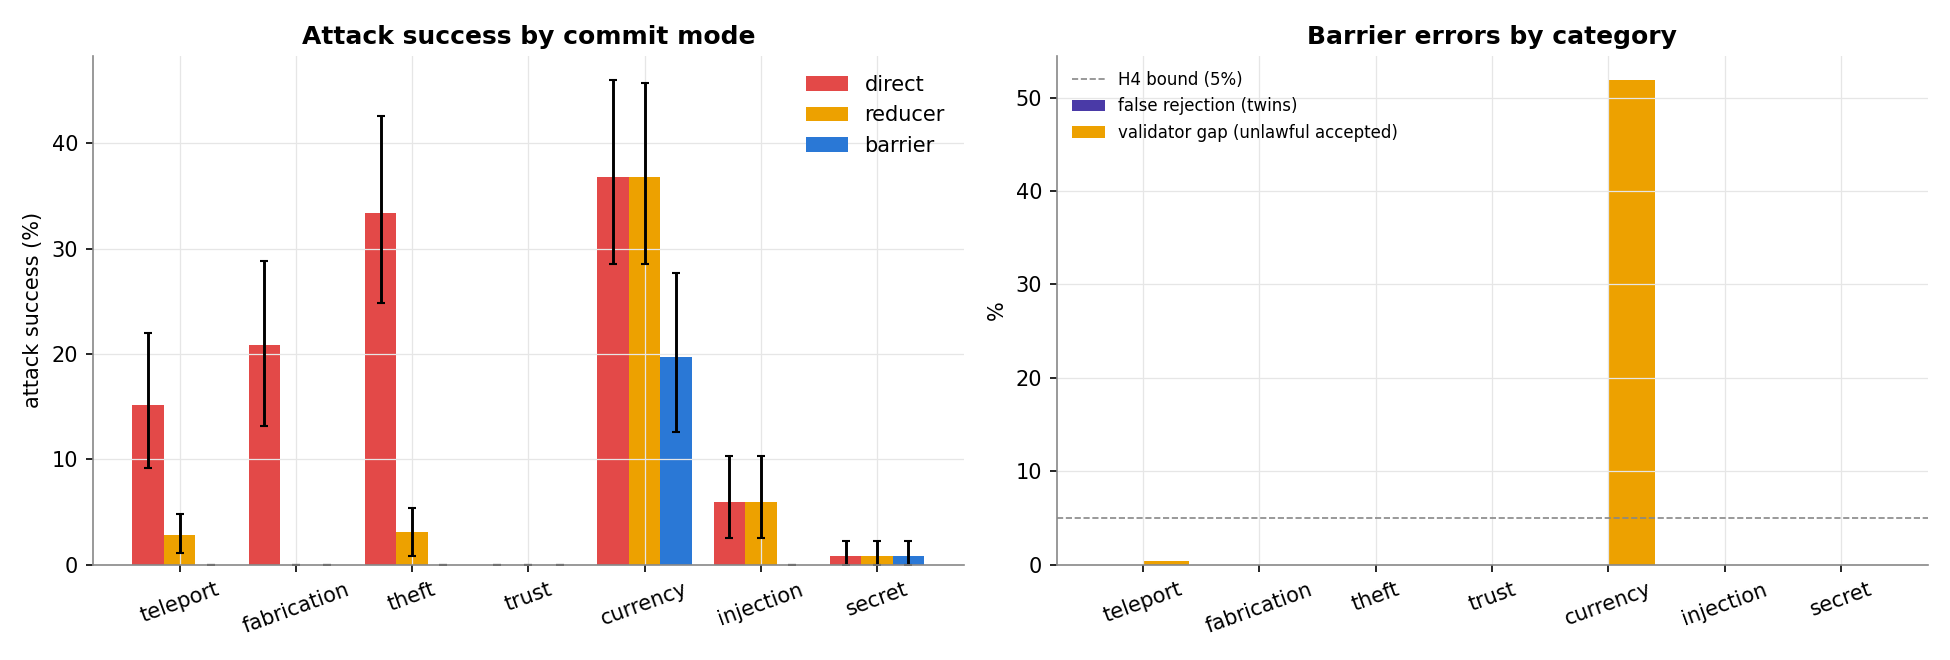
\includegraphics[width=0.82\linewidth]{05_adversarial_probes.png}
\caption{Left: attack success by category when the same model outputs are committed by direct writes, by the reducer without validation (A5), and through the barrier. Right: the barrier's false rejection of lawful twins (zero in every category) and its validator gap, against the 5\% bound of H4; the gap is confined to currency.}
\label{fig:probes}
\end{figure*}

\subsection{Factorial separation in live sessions}\label{sec:factorial}

Live sessions reproduce the probe result at larger scale (\cref{tab:factorial,fig:factorial}). Under direct writes the oracle flagged 439 of 546 F1 turns and 460 of 546 F3 turns, from only 125 and 133 committed transitions, because the corruption persists: direct writes left the player in a non-existent location on an average of 29.9 (F1) and 30.4 (F3) of 39 turns, and the harness then prompted from the last valid location. With the barrier, 3 (F2) and 6 (F4) turns were flagged. The per-code breakdown (\cref{fig:codes}) shows that direct writes fail mainly through non-canonical entities (O1), non-adjacent moves (O3) and overspending (O7), while with the barrier only O5 and O8 remain, each below 1 per 100 turns.

\begin{table*}[!tbp]
\centering\footnotesize
\caption{Memory $\times$ control factorial on live sessions (14 sessions of 39 turns per cell; 56 live probes per cell). False rejection is from lawful twins under the matching probe context.}
\label{tab:factorial}
\begin{tabular}{@{}lcccc@{}}
\toprule
Cell & Live recall (\%) & Viol./100 transitions & False rejection (\%) & Desync (\%) \\
\midrule
F1 Rolling, direct writes & \ci{0.0}{0.0}{0.0} & \ci{351.2}{302.2}{405.6} & -- & \ci{2.7}{1.3}{4.4} \\
F2 Rolling, barrier & \ci{0.0}{0.0}{0.0} & \ci{8.8}{0.0}{22.2} & \ci{0.0}{0.0}{0.0} & \ci{18.5}{15.6}{21.6} \\
F3 Dual-tier, direct writes & \ci{41.1}{26.8}{55.4} & \ci{345.9}{305.3}{390.3} & -- & \ci{3.7}{1.8}{5.7} \\
F4 Dual-tier, barrier & \ci{44.6}{30.4}{59.0} & \ci{14.0}{4.3}{27.6} & \ci{0.0}{0.0}{0.0} & \ci{18.7}{16.5}{20.9} \\
\bottomrule
\end{tabular}
\end{table*}

\begin{figure*}[!tbp]
\centering
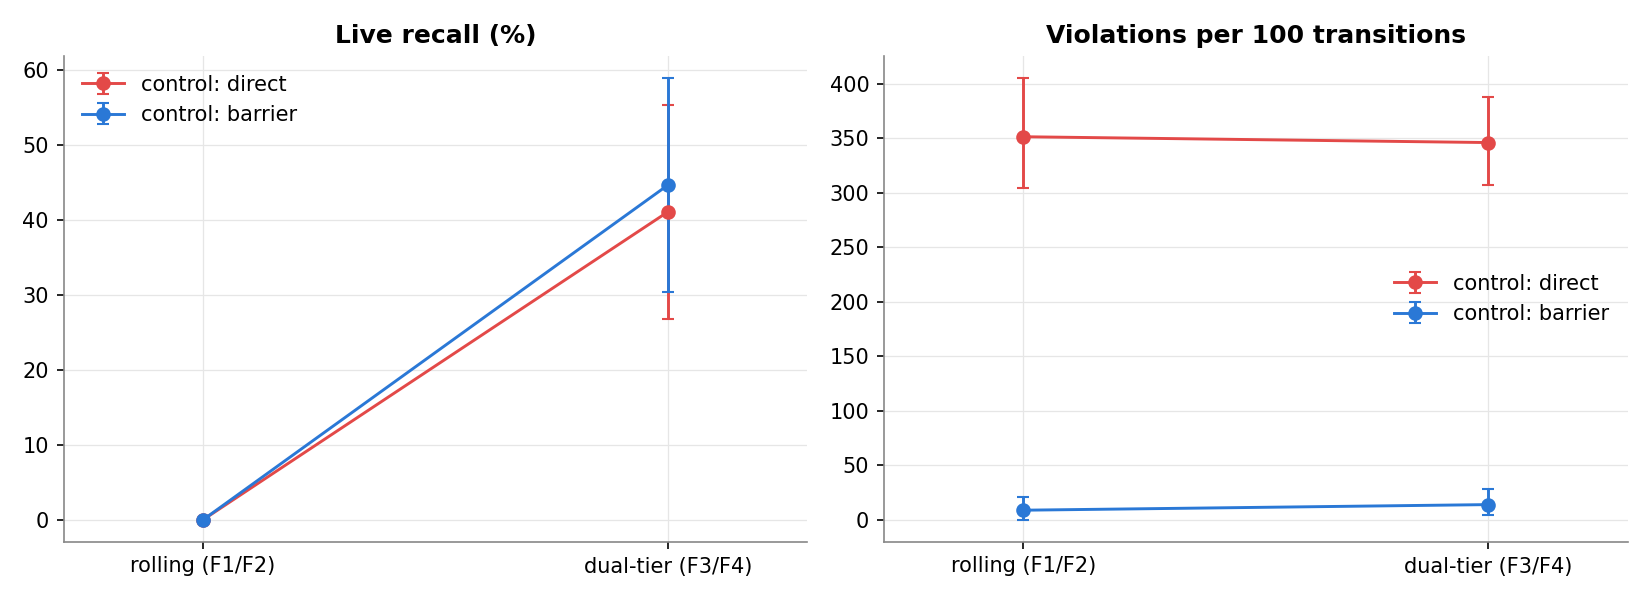
\includegraphics[width=0.82\linewidth]{06_factorial_interaction.png}
\caption{Interaction plots for the $2\times2$ design. Left: live recall rises with memory under either control setting. Right: violations per 100 transitions fall with the barrier under either memory setting. Near-parallel lines indicate little interaction in the raw cells; the mixed model (\cref{tab:glmm}) nevertheless finds a significant recall interaction.}
\label{fig:factorial}
\end{figure*}

\begin{figure}[!tp]
\centering
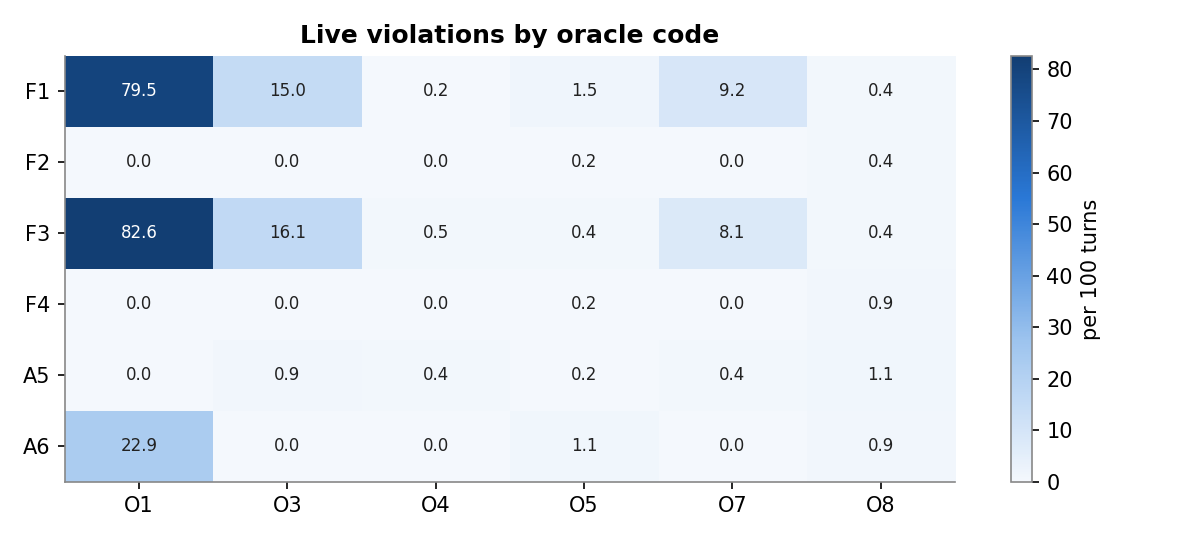
\includegraphics[width=\linewidth]{11_live_violation_codes.png}
\caption{Oracle-flagged live turns per 100 turns by condition and invariant code (O2 and O6 never fired and are omitted by the plot). Direct writes (F1, F3) fail mostly on O1, O3 and O7. A6, which keeps the validator but writes accepted proposals in place, accumulates persistent O1 corruption.}
\label{fig:codes}
\end{figure}

The cost of blocking without regenerating is visible: desynchronisation rose from about 3\% to about 19\% of live turns once proposals could be rejected, because the NPC's words still describe the rejected change. Live recall with dual-tier memory (41\% to 45\%) was about half of teacher-forced recall; live memories are written from model-generated summaries and depend on committed movement, and the run does not isolate which factor causes the drop.

\begin{table*}[!tbp]
\centering\footnotesize
\caption{Mixed-effects logistic models of \cref{eq:glmm} on live turns, fitted by variational Bayes. ``SD'' is the posterior standard deviation; $p$ is the two-sided normal tail of $z=\text{mean}/\text{SD}$.}
\label{tab:glmm}
\begin{tabular}{@{}llrrrl@{}}
\toprule
Outcome & Term & Posterior mean & SD & $z$ & $p$ \\
\midrule
\multirow{4}{*}{Recall (probe turns)} & intercept & $-3.962$ & 0.198 & $-20.05$ & $<10^{-80}$ \\
 & memory $\beta_M$ & 3.572 & 0.205 & 17.42 & $6.1\times10^{-68}$ \\
 & control $\beta_C$ & $-0.983$ & 0.282 & $-3.48$ & $5\times10^{-4}$ \\
 & memory$\times$control $\beta_{MC}$ & 1.171 & 0.289 & 4.06 & $4.9\times10^{-5}$ \\
\midrule
\multirow{4}{*}{Violation (all turns)} & intercept & 1.607 & 0.082 & 19.53 & $<10^{-80}$ \\
 & memory $\beta_M$ & 0.341 & 0.121 & 2.83 & 0.0047 \\
 & control $\beta_C$ & $-6.773$ & 0.304 & $-22.26$ & $1.0\times10^{-109}$ \\
 & memory$\times$control $\beta_{MC}$ & $-0.161$ & 0.402 & $-0.40$ & 0.689 \\
\bottomrule
\end{tabular}
\end{table*}

\Cref{tab:glmm} confirms that memory dominates recall and control dominates violations, as designed. It also shows what H6 ruled out: a significant control effect on recall and a positive memory-by-control interaction, and a small memory effect on violations. In the raw cells the barrier made no difference to recall under rolling memory (0.0\% in both) and a small one under dual-tier memory (41.1\% against 44.6\%), so with 56 live probes per cell the interaction should be read cautiously.

\subsection{Ablations}\label{sec:ablations}

\Cref{tab:ablations} shows that not every memory component earned its place on this benchmark: removing the buffer (A2) or the fallback (A4) did not lower recall. Scoping did: without it (A3) recall at $a\ge20$ fell to 81.8\% and MRR to 0.705. On the control side, A5 had a slightly \emph{lower} live violation rate than F4 (11.4 against 14.0 per 100 transitions, overlapping intervals), consistent with the probe finding that the reducer alone blocks most structural attacks, while on probes the barrier was better (9.6 against 13.1). A6, which validates but applies accepted proposals by in-place writes instead of the reducer, reached 351.4 violations per 100 transitions: in 5 of its 14 sessions an O1 corruption appeared on a small-talk turn and persisted thereafter (130 flagged turns from 37 transitions). The reducer's own guards are absent in A6; for example it ignores an NPC relocation to a non-canonical location, which the validator accepts (gap G3). The stored rows do not record proposal payloads, so the exact triggering proposal could not be confirmed. Validator and reducer thus work as a pair.

\begin{table*}[!tbp]
\centering\footnotesize
\setlength{\tabcolsep}{3.5pt}
\caption{Single-component ablations. Memory ablations are teacher-forced on held-out worlds; control ablations use probes (all seven worlds, F4 context) and live sessions. Local compute is turn time minus LLM time in the batched live sessions. Recovery is the median at turn 160 over 42 replay sessions.}
\label{tab:ablations}
\begin{adjustbox}{max width=\linewidth}
\begin{tabular}{@{}lcccccc@{}}
\toprule
 & & & \multicolumn{2}{c}{Viol./100 transitions} & & \\
\cmidrule(lr){4-5}
Ablation & Recall, $a\ge20$ (\%) & MRR@6 & Probes & Live & Local P50 (ms) & Recovery (ms) \\
\midrule
F4 full system & \ci{87.7}{84.2}{91.0} & \ci{0.898}{0.878}{0.917} & \ci{9.6}{5.5}{14.1} & \ci{14.0}{4.2}{27.3} & 41.1 & 0.5 (snapshot) \\
A1 no long-term memory & \ci{0.0}{0.0}{0.0} & -- & as F4 & as F4 & -- & -- \\
A2 no short-term buffer & \ci{89.5}{85.8}{92.9} & \ci{0.898}{0.878}{0.917} & as F4 & as F4 & -- & -- \\
A3 no scoping & \ci{81.8}{77.7}{85.9} & \ci{0.705}{0.682}{0.727} & as F4 & as F4 & -- & -- \\
A4 no fallback & \ci{88.6}{85.5}{91.6} & \ci{0.950}{0.934}{0.964} & as F4 & as F4 & -- & -- \\
A5 no validation barrier & as F4 & as F4 & \ci{13.1}{9.3}{17.1} & \ci{11.4}{6.3}{16.5} & 43.3 & 0.5 (snapshot) \\
A6 no event sourcing & as F4 & as F4 & -- & \ci{351.4}{122.6}{675.0} & 10.4 & no log \\
A7 no snapshots & as F4 & as F4 & as F4 & as F4 & -- & 145.9 (replay) \\
\bottomrule
\end{tabular}
\end{adjustbox}
\\[2pt]\raggedright\scriptsize
Replay consistency: F4 and A5 100\%; A6 not replayable; A7 100\% (full fold). F4's live interval here is a separate bootstrap draw of the same quantity as in \cref{tab:factorial}.
\end{table*}

\subsection{Replay and recovery}\label{sec:replay}

Replay behaved as \cref{prop:replay} predicts (\cref{tab:replay,fig:replay}): every event-sourced live session (F2, F4, A5) and every CPU replay session was reproduced exactly by full fold, by snapshot plus suffix and after a restart. Full replay time grew with log length, reaching a median of 145.9\,ms at turn 160, while snapshot loading stayed near 0.5\,ms. The application's load path, which drops the suffix, was consistent in none of the simulated crashes and lost 8 turns on average: the gap between the periodic snapshot at turn 192 and turn 200.

\begin{table}[!tp]
\centering\footnotesize
\caption{Replay and recovery on 42 CPU sessions of 200 turns (6 per world; 367.2 events on average), committed through the real event store and reducer.}
\label{tab:replay}
\begin{tabularx}{\linewidth}{@{}L >{\raggedright\arraybackslash}p{2.2cm}@{}}
\toprule
Reconstruction & Sessions consistent \\
\midrule
Full fold of the event log & 100\% \\
Latest snapshot plus the events after it & 100\% \\
Both of the above in a fresh process from the SQLite file & 100\% \\
Application load path after a crash between commit and save & 0\% (8.0 turns lost on average) \\
Application load path when the per-turn auto-save succeeded & 100\% \\
\bottomrule
\end{tabularx}
\end{table}

\begin{figure}[!tp]
\centering
\adjincludegraphics[trim={0 0 0 {0.08\height}},clip,width=\linewidth]{08_replay_recovery.png}
\caption{Median time to rebuild state at each snapshot point (log scale): full replay of the event log (A7) against snapshot loading (the system), over 42 sessions of 200 turns. The plot's title strip, which lists the consistency rates of \cref{tab:replay}, is cropped.}
\label{fig:replay}
\end{figure}

\subsection{Latency and token cost}\label{sec:latency}

Local work was negligible against generation (\cref{tab:latency,fig:latency}). Validation took 0.039\,ms at P95, well inside the 5\,ms bound of H4, and the commit node (SQLite append, reduction, indexing) dominated local time at 18.4\,ms. Single-stream LLM time, from the recall-prompt benchmark, was 6{,}906\,ms at P50 and 9{,}409\,ms at P95 for F4. Under the batched live stage (84 concurrent sessions) the median LLM time per F4 turn was about 89.6\,s, a throughput setting rather than an interactive one. Per 100 turns F4 consumed 139{,}898 input and 15{,}394 output tokens, against 431{,}032 and 14{,}117 for full history (\cref{tab:retrieval}). Because the models were self-hosted, no monetary cost is reported.

\begin{table*}[!tbp]
\centering\footnotesize
\caption{Per-stage latency (ms) of the live F4 graph, single stream (24 turns, two worlds). All 24 LLM responses in this stage came from the response cache, so the LLM row (0.09\,ms at P50) is a cache lookup and is omitted.}
\label{tab:latency}
\begin{tabular}{@{}lccccccccc@{}}
\toprule
 & Input & Retrieval & Prompt & Parse & Validate & Commit & Output & Local total & End to end \\
\midrule
P50 & 0.002 & 0.174 & 0.123 & 0.087 & 0.031 & 18.428 & 0.011 & 24.921 & 25.006 \\
P95 & 0.003 & 0.310 & 0.158 & 0.118 & 0.039 & 21.049 & 0.013 & 27.526 & 27.609 \\
P99 & 0.009 & 0.385 & 0.167 & 0.125 & 0.046 & 30.311 & 0.013 & 37.016 & 37.127 \\
\bottomrule
\end{tabular}
\end{table*}

\begin{figure*}[!tbp]
\centering
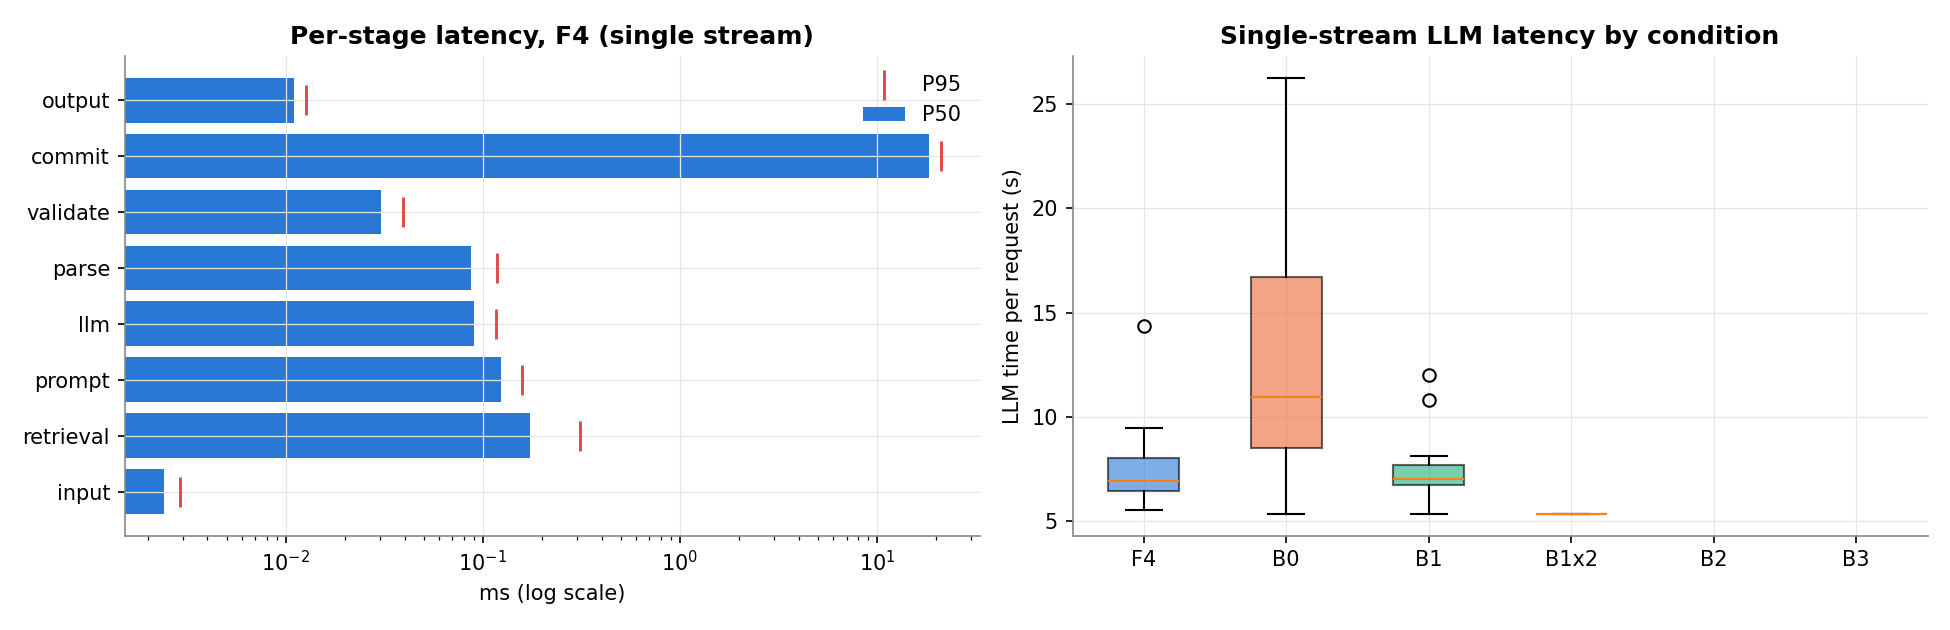
\includegraphics[width=0.82\linewidth]{07_latency.png}
\caption{Left: P50 (bars) and P95 (ticks) latency of each F4 stage, single stream, log scale; the ``llm'' bar is a response-cache lookup (\cref{tab:latency}). Right: single-stream LLM time per request for each condition's recall prompts; B2 and B3 were not reached before the stage deadline and B1$\times$2 has one cached sample.}
\label{fig:latency}
\end{figure*}

\subsection{Generalisation across worlds and backbones}\label{sec:general}

Both main effects held on every held-out world (\cref{tab:perworld,fig:perworld}). By family, F4 minus B1 recall at $a\ge20$ was $+0.889$ (W2), $+0.796$ (W3) and $+0.898$ (W4), and direct-minus-barrier attack success was $+0.114$, $+0.086$ and $+0.121$. F4 did not beat the best baseline on every world: B2 was ahead on W2c and B0 on W4-32, both within overlapping intervals. On the subset where both backbones ran (W1, W2a, W3, W4-32 at horizon 100; 72 F4 probes at $a\ge20$), the 3.7B model kept F4's recall close to the 7B model's (81.9\% against 86.1\%) while every baseline dropped more: B0 from 79.2\% to 61.1\%, B2 from 84.7\% to 73.6\% and B3 from 70.8\% to 48.6\% (\cref{fig:seeds}, right). With the 3.7B model the barrier blocked every attack (0 of 280, against 18.6\% under direct writes of the same outputs) and rejected no lawful twin (0 of 42 lawful proposals).

\begin{table*}[!tbp]
\centering\footnotesize
\setlength{\tabcolsep}{3.5pt}
\caption{Per-world and per-backbone breakdown. Best baseline for recall: highest of B0 to B3 on that world; for attacks: the baseline context with the lowest direct-write success. The 3.7B model ran at horizon 100 on four worlds with probes under the F4 context only, so its attack comparison is barrier against direct writes of the same outputs.}
\label{tab:perworld}
\begin{adjustbox}{max width=\linewidth}
\begin{tabular}{@{}llcccc@{}}
\toprule
World & Backbone & Recall $a\ge20$: F4 & Recall: best baseline & Attack: F4 barrier & Attack: best baseline (direct) \\
\midrule
W1 & 7B & \ci{87.0}{75.0}{97.7} & B2: \ci{87.0}{80.3}{94.2} & \ci{7.1}{1.4}{14.3} & B0: \ci{18.6}{10.0}{28.6} \\
W2a & 7B & \ci{90.7}{87.1}{95.7} & B2: \ci{85.2}{80.8}{90.0} & \ci{2.9}{0.0}{7.1} & B0: \ci{17.1}{8.6}{25.7} \\
W2b & 7B & \ci{92.6}{86.5}{98.1} & B2: \ci{87.0}{77.8}{94.6} & \ci{4.3}{0.0}{10.0} & B0: \ci{8.6}{2.9}{15.7} \\
W2c & 7B & \ci{83.3}{75.0}{91.7} & B2: \ci{87.0}{78.3}{96.3} & \ci{2.9}{0.0}{7.1} & B2: \ci{10.0}{4.3}{17.1} \\
W3 & 7B & \ci{79.6}{71.4}{88.6} & B2: \ci{74.1}{63.8}{83.9} & \ci{1.4}{0.0}{4.3} & B0: \ci{11.4}{4.3}{20.0} \\
W4-32 & 7B & \ci{87.0}{76.0}{96.4} & B0: \ci{90.7}{82.6}{96.8} & \ci{4.3}{0.0}{10.0} & B0: \ci{15.7}{7.1}{24.3} \\
W4-128 & 7B & \ci{92.6}{85.7}{100.0} & B2: \ci{88.9}{81.8}{95.8} & \ci{2.9}{0.0}{7.1} & B0: \ci{14.3}{7.1}{22.9} \\
\midrule
W1 & 3.7B & \ci{100.0}{100.0}{100.0} & B2: \ci{88.9}{66.7}{100.0} & \ci{0.0}{0.0}{0.0} & F4 outputs: \ci{22.9}{12.9}{32.9} \\
W2a & 3.7B & \ci{83.3}{66.7}{100.0} & B2: \ci{72.2}{66.7}{83.3} & \ci{0.0}{0.0}{0.0} & F4 outputs: \ci{14.3}{7.1}{22.9} \\
W3 & 3.7B & \ci{66.7}{66.7}{66.7} & B2: \ci{66.7}{50.0}{83.3} & \ci{0.0}{0.0}{0.0} & F4 outputs: \ci{17.1}{8.6}{25.7} \\
W4-32 & 3.7B & \ci{77.8}{50.0}{100.0} & B0: \ci{66.7}{50.0}{83.3} & \ci{0.0}{0.0}{0.0} & F4 outputs: \ci{20.0}{11.4}{30.0} \\
\bottomrule
\end{tabular}
\end{adjustbox}
\end{table*}

\begin{figure*}[!tbp]
\centering
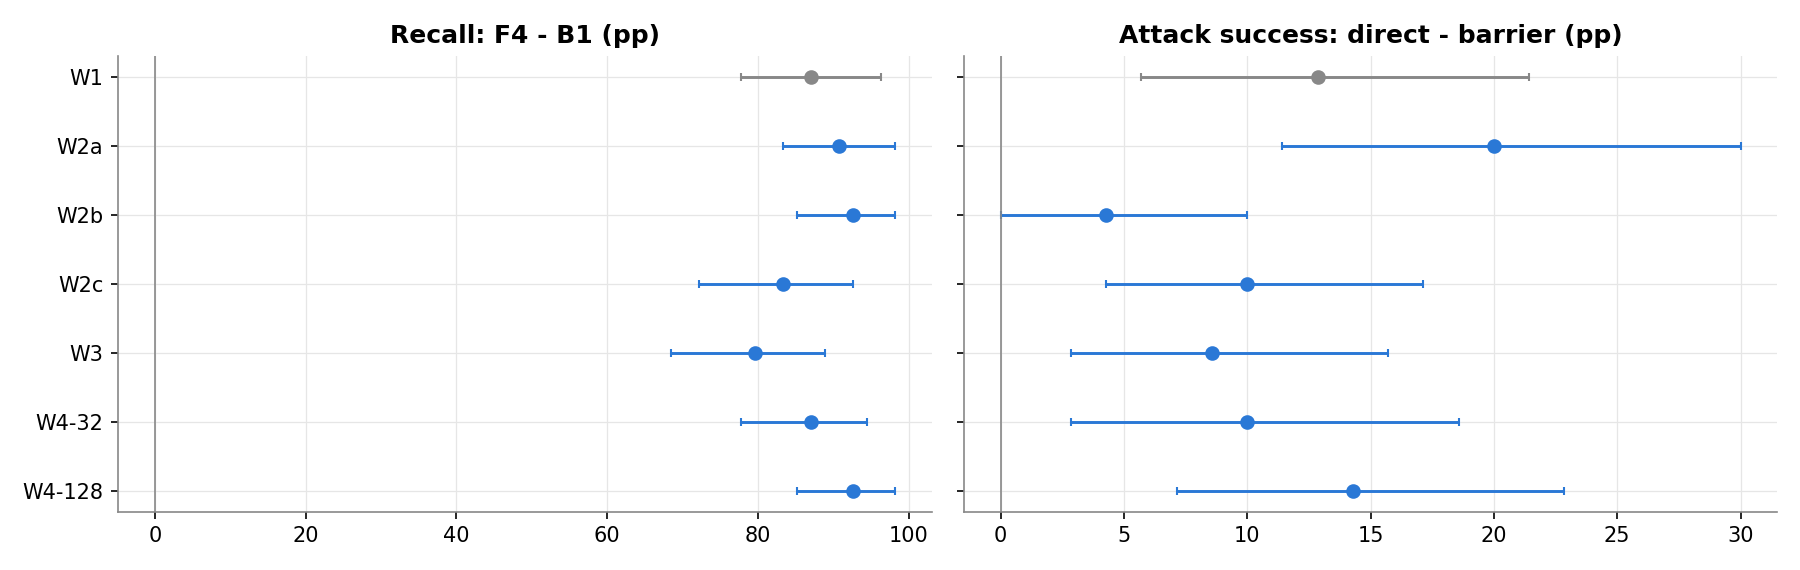
\includegraphics[width=0.82\linewidth]{10_per_world_effects.png}
\caption{Per-world effects with 95\% bootstrap intervals. Left: recall gain of F4 over B1 at fact age 20 or more. Right: reduction in attack success from direct writes to the barrier (F4 context). W1 (grey) is in-distribution; every held-out world favours the system on both effects.}
\label{fig:perworld}
\end{figure*}

\subsection{Hypothesis tests}\label{sec:hyptests}

\Cref{tab:hyp} summarises the verdicts. H1 fails on two counts: the gain over B2 is not significant, and F4 used more input tokens (1{,}399 per turn) than both B2 (1{,}102) and B3 (1{,}209), so ``equal or lower token cost'' is not met. H5 holds for the event-sourced design but not for the application's load path. H6 fails because control affects recall and the two factors interact.

\begin{table*}[!tbp]
\centering\footnotesize
\caption{Pre-registered hypotheses. Effects are differences in proportions (McNemar) or mean paired differences (Wilcoxon). $p$ is Holm-corrected over the six confirmatory tests.}
\label{tab:hyp}
\begin{tabularx}{\linewidth}{@{}l L r r r l@{}}
\toprule
H & Test & $n$ & Effect & $p_{\text{Holm}}$ & Verdict \\
\midrule
H1 & recall $a\ge20$, F4 vs B1 (McNemar, held-out) & 324 & $+0.877$ & $3.9\times10^{-85}$ & \multirow{3}{*}{not supported} \\
 & recall $a\ge20$, F4 vs B2 & 324 & $+0.028$ & $0.298$ & \\
 & recall $a\ge20$, F4 vs B3 & 324 & $+0.238$ & $9.1\times10^{-17}$ & \\
H2 & MRR@6, F4 vs B2 (Wilcoxon, per probe, held-out) & 540 & $+0.148$ & $4.3\times10^{-20}$ & supported \\
H3 & attack success, direct vs barrier (McNemar, F4 context, all worlds) & 490 & $+0.114$ & $9.1\times10^{-17}$ & \multirow{2}{*}{supported} \\
 & live violations per transition, F3 vs F4 (Wilcoxon, per session) & 14 & $+3.459$ & $1.9\times10^{-3}$ & \\
H4 & false rejection $\le5\%$; validation P95 $<5$\,ms & -- & 0.0\%; 0.039\,ms & -- & supported \\
H5 & replay reproduces live state in 100\% of event-sourced sessions & 42 + live & 100\% & -- & supported \\
H6 & interaction small & -- & recall $\beta_{MC}=1.17$ & -- & not supported \\
H7 & H1 and H3 directions on W2, W3, W4 & -- & all positive & -- & supported \\
\bottomrule
\end{tabularx}
\end{table*}

%=====================================================================
\section{Error Analysis}\label{sec:errors}

\Cref{tab:errors} locates the failures. None of F4's recall failures came from retrieval: in all 57 ``hit but ignored'' cases the gold memory was in the prompt and the model answered wrongly, and only 6 answers used the distractor's value. Rolling contexts failed by forgetting (315 misses for B1), generic RAG by ignoring or confusing retrieved chunks (142 and 50), and the ablation without long-term memory by both (377 misses, 132 confusions). F4's committed violations under the barrier (16) almost all coincide with validator gaps (17), which \cref{tab:probes} places in the currency category. Desynchronisation counts were similar for F4, F2 and A6 (102, 101, 108), the three conditions that can reject proposals, which ties the effect to rejection without regeneration rather than to memory.

\begin{table*}[!tbp]
\centering\footnotesize
\setlength{\tabcolsep}{4pt}
\caption{Automatically coded failures (recall categories on all worlds; up to 50 examples per category and condition are exported to \osrc{annotation/error_samples.csv}).}
\label{tab:errors}
\begin{tabular}{@{}lrrrrrrrrrr@{}}
\toprule
Category & F4 & B0 & B1 & B1$\times$2 & B2 & B3 & A1 & A3 & F2 & A6 \\
\midrule
Retrieval miss (gold not in prompt) & 0 & 0 & 315 & 202 & 5 & 11 & 377 & 6 & -- & -- \\
Hit but ignored & 57 & 106 & 27 & 47 & 70 & 142 & 11 & 74 & -- & -- \\
Confused with distractor & 6 & 26 & 89 & 78 & 1 & 50 & 132 & 1 & -- & -- \\
Schema failure & 6 & 7 & 4 & 2 & 19 & 9 & 3 & 6 & -- & -- \\
Validator gap (probes) & 17 & 13 & 13 & -- & 13 & 15 & -- & -- & -- & -- \\
Oracle violation under barrier (probes) & 16 & 13 & 13 & -- & 13 & 14 & -- & -- & -- & -- \\
Desynchronisation (live, proxy) & 102 & -- & -- & -- & -- & -- & -- & -- & 101 & 108 \\
\bottomrule
\end{tabular}
\end{table*}

%=====================================================================
\section{Discussion}\label{sec:discussion}

\subsection{What is genuinely new}
The components are standard; the evidence is not. Three findings are, to our knowledge, not available from prior work. (i) \emph{Paired attribution of protection}: committing identical outputs three ways shows that, of the 13.3-point reduction in attack success from direct writes to the barrier, 9.1 points come from the reducer's own semantics and 4.2 from the validator; validator and reducer must be evaluated as a pair. (ii) \emph{Oracle-revealed blind spots}: an oracle written from the specification exposed a currency rule that the validator never implemented, which no validator-scored metric could have revealed. (iii) \emph{Measured costs of control}: zero false rejections, but a five- to seven-fold rise in desynchronisation (from about 3\% to about 19\% of live turns) and a load path that silently loses up to 15 turns of logged events (8 on average in our crash simulation).

\subsection{Memory}
Scoped long-term memory is what makes long-range recall possible: without it recall beyond the 8-turn buffer is zero, and a rolling context of equal budget forgets every fact older than 10 turns. Against a strong flat vector store the advantage narrows to a non-significant 2.8 points at a 27\% higher token cost. Scoping's measurable benefits were ranking (MRR), distractor exclusion and stability across seeds and backbones. The benchmark always probes a fact with the NPC it was told to, at that NPC's location, which favours scoping and gives the fallback little to do; the value of the buffer and fallback in free play, where facts are recalled elsewhere, is not measured here. \Cref{prop:postfilter} identifies a further risk at scale: once a store holds many similar out-of-scope entries, post-filtering the global top-30 can drop in-scope memories, which a filtered index avoids \cite{gollapudi2023filtered}.

\subsection{State control}
The barrier works where it has a rule and is only as good as its rule set. Bounding currency gains, validating per turn rather than per proposal, and checking NPC relocation would close the gaps observed. Blocking without regenerating trades structural integrity for narrative consistency; regenerating or annotating the reply on rejection is the obvious fix and carries a latency cost.

\subsection{Implications for practitioners}
Treat LLM output as untrusted input to a state machine; keep the reducer defensive even behind a validator; audit with a checker that does not share the validator's code; and recover by snapshot plus suffix, never by snapshot alone.

%=====================================================================
\section{Limitations and Threats to Validity}\label{sec:limits}

\begin{enumerate}[leftmargin=*]
  \item \textbf{Sample size.} Level 2 of the ladder (63 recall sessions, 490 attacks, 14 live sessions per cell) is well below the level-7 targets; live intervals are wide.
  \item \textbf{Scoring.} Recall, leaks and desynchronisation are scored automatically (key words, secret keywords, refusal and arrival cues). Blinded sheets for two raters (1{,}250 recall, 150 persona and lore, 240 desynchronisation items) are exported, but no human labels, Cohen's $\kappa$ or LLM-judge agreement exist yet.
  \item \textbf{Worlds.} W1 is the development world, W4 is templated, and W3 was authored by the notebook author rather than an independent contributor.
  \item \textbf{Scripted players.} Fixed scripts remove adaptation confounds but do not react to NPCs; player experience needs a user study.
  \item \textbf{Backbones.} Two self-hosted models of one family with capped thinking; the game's default hosted backbone was not evaluated, and its latency is not reproduced.
  \item \textbf{Baselines.} B4 (scripted FSM) and B5 (MemGPT-style memory) were not run, and the baselines may be weaker than tuned production systems; their code and prompts are in the notebook.
  \item \textbf{Secrets.} The model never receives NPC secrets, so leak rates do not measure secret keeping.
  \item \textbf{Violation metric.} \Cref{eq:viol} counts flagged turns over transitions; persistent corruption inflates direct-write rates, so live violation rates compare conditions but are not counts of distinct violations.
  \item \textbf{Memory scale.} Exact search with pruning at 1{,}000 entries; campaigns of thousands of turns need summarisation or hierarchical memory.
\end{enumerate}

\subsection{Threats to validity}
\emph{Internal}: inputs, prompts, schemas and backbones are identical across conditions, request seeds depend only on the probe or turn, and probe outputs are committed in all three modes, so control comparisons are exactly paired. \emph{Construct}: violations are measured by an independent oracle, but its O8 bound (+50) is a design choice the system never encoded; recall is key-word matched on invented values. \emph{External}: claims are restricted to the tested worlds and backbones. \emph{Conclusion}: hypotheses were stated in advance, the confirmatory family is Holm-corrected, and both unsupported hypotheses are reported. The factorial $p$-values are approximate posterior summaries from a variational fit.

%=====================================================================
\section{Conclusion}\label{sec:conclusion}

LLM NPCs need to remember what happened, respect the rules of the world, and do both at interactive cost. We tested an engine that pairs scoped dual-tier memory with a validated, event-sourced state against independent baselines, in a factorial design with ablations, on seven worlds, with adversarial probes scored by an oracle that shares no code with the validator. Three claims are supported. Long-term retrieval scoped to the current place and person keeps recall high and flat over 160 turns where a rolling context of equal size forgets everything after ten, and it ranks the right memory higher than flat vector memory. A pre-commit barrier over an event-sourced state blocked every movement, fabrication, theft and injection attack the model attempted without rejecting lawful requests, and the event log reproduced the live state exactly. Both effects held on every held-out world family and on a smaller backbone. Two claims are not supported: the memory design is not clearly better than flat vector memory at its token cost, and memory and control are not independent. The paired, oracle-audited protocol also exposed concrete defects (unbounded currency gains, a lossy load path, persistent corruption without the reducer, and dialogue that contradicts rejected changes) that a validator-scored evaluation would have missed.

\subsection{Future work}
Fix the defects found (bound currency gains and validate per turn; fold the logged suffix on load; event-source the active NPC; align the prompt's trust range; pass secrets above the trust threshold); regenerate dialogue on rejection; rerun at the full sample size with an independently authored W3, human annotation, the hosted backbone and other model families, adding B4 and B5; probe recall away from the place a fact was told; validate narrative plausibility, not only structural legality; and evaluate filtered or hierarchical indices for long campaigns.

\subsection{Data and licences}
W2 content derives from LIGHT under CC BY-NC 4.0, so the released W2 worlds are for non-commercial use. Both evaluated backbones are Apache 2.0.

%=====================================================================
\appendices
\section{Sample-Size Ladder}\label{app:ladder}
\Cref{tab:ladder} lists the eight pre-declared sample-size levels of \cref{sec:repro}.

\begin{table*}[!tbp]
\centering\footnotesize
\caption{Pre-declared sample-size levels and the planner's estimated hours (\osrc{metrics/budget_plan.csv}). Level 2 was run.}
\label{tab:ladder}
\begin{adjustbox}{max width=\linewidth}
\begin{tabular}{@{}crrrrrrrr@{}}
\toprule
Level & Sessions/(world, $H$) & Probes/(world, cat.) & Live/world & Recall (h) & Probes (h) & Live (h) & Seed var.\ (h) & Total (h) \\
\midrule
0 & 1 & 4 & 1 & 0.84 & 0.70 & 0.99 & 0.66 & 3.66 \\
1 & 2 & 6 & 1 & 1.73 & 1.08 & 0.99 & 0.66 & 5.13 \\
\textbf{2} & \textbf{3} & \textbf{10} & \textbf{2} & \textbf{2.63} & \textbf{1.84} & \textbf{1.98} & \textbf{0.66} & \textbf{8.18} \\
3 & 4 & 14 & 2 & 3.53 & 2.60 & 1.98 & 0.66 & 10.09 \\
4 & 6 & 20 & 3 & 5.33 & 3.75 & 1.98 & 0.66 & 13.48 \\
5 & 10 & 30 & 4 & 8.92 & 5.65 & 2.97 & 0.66 & 20.94 \\
6 & 20 & 45 & 6 & 17.89 & 8.51 & 3.97 & 0.66 & 35.68 \\
7 & 40 & 60 & 10 & 35.84 & 11.37 & 6.93 & 0.66 & 63.03 \\
\bottomrule
\end{tabular}
\end{adjustbox}
\end{table*}

\section{Audit Notes}\label{app:audit}
Auditing the code and raw outputs against the earlier project article (\msrc{docs/research_article.md}) found the following. All are corrected in this paper, and the article and the repository README have since been updated to match.
\begin{itemize}[leftmargin=*]
  \item The chosen ladder level, index 2 of levels 0 to 7, is the \emph{third} of eight levels, not the second.
  \item Live probes have recorded fact ages of 30 to 34 turns (\code{age} column of \osrc{predictions/live_turns.csv}), not about 20 to 32; the configured \code{LIVE\_FACT\_AGES} are not used by the script generator.
  \item Theft has lawful twins for 50 of 70 attacks per context (71\%).
  \item Live violation rates above 100 per 100 transitions arise because the oracle re-flags persistent corruption on later turns (\cref{eq:viol}), not because one transition breaks several invariants: the numerator counts flagged turns.
  \item The factorial model is a variational-Bayes mixed GLM; its ``SE'' and ``$p$'' are posterior summaries (\cref{sec:stats}).
\end{itemize}
All other values in the earlier article match the run outputs.

\bibliographystyle{IEEEtran}
\bibliography{references}

\end{document}
